% DSXL_3_doc_and_exercices_CREATION_EXERCICE.tex

La création d'un exercice se fait avec le programme dsxl\_3\_exercice\_creation.py.

A l'ouverture du programme trois onglets se présentent :

\begin{figure}[h]
 \centering
 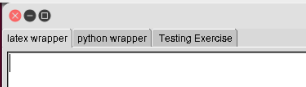
\includegraphics{./images/creation_exercice_01.png}
 % creation_exercice_01.png: 306x87 px, 96dpi, 8.10x2.30 cm, bb=0 0 229 65
 \caption{Onglets dans le programme de création des exercices}
 \label{fig:01}
\end{figure}

La création d'un exercice passe par l'utilisation successive de ces trois onglets. 

\section{L'onglet \underline{latex wrapper}}

\subsection{Etape 1 : Entrer le code Latex}
Coller le code Latex dans la zone de texte à gauche. Il est important que, déjà à ce stade la solution soit aussi rédigée. 

L'exemple que nous allons prendre sera celui d'une étude de fonction quadratique. L'exercice aura deux parties : 
\begin{description}
 \item[Partie A :] Lecture graphique et
 \item[Partie B :] Calcul d'image et d'antécédent (donc résolution d'une équation)
\end{description}

\begin{remarque}
 Pour la partie graphique, le plus simple est d'utiliser le programme GeoGebra pour générer le code PGF/TikZ et de l'adapter. 
\end{remarque}
 
 \begin{remarque}
 Tout exercice commence par la commande \index[dsxlindex]{$\backslash$EXERCICE} . 
\end{remarque}
 
\begin{dsxl}
 Dans l'onglet \underline{Latex wrapper}, le \index[dsxlindex]{bouton \fbox{WRAP UP!}} effectue les actions suivantes :
 \begin{enumerate}
  \item Sauvegarde la zone de texte à gauche dans le fichier :\\
   {\bf DSXL\_3\_programme/dsxl\_tex\_exercice/dsxl\_text\_latex\_wrapper\_in.tex}. 
   \item Génère le code Latex complet qui se trouvera dans le fichier : \\
 {\bf DSXL\_3\_programme/dsxl\_tex\_exercice/latex\_wrapper\_in\_full/dsxl\_text\_latex\_wrapper\_in.tex}. 
 \item Remplace les \index[dsxlindex]{balises $\%E>$ (début énoncé)  $\%E<$ (fin énoncé),  $\%C>$ (début corrigé)  $\%C<$ (fin corrigé)},  insérées dans la zone de texte à gauche par l'équivalent commande Latex.  
  
 \end{enumerate}

 
 
 Il est important de travailler de manière incrémentielle : 
 \begin{description}
  \item [1.] Ajouter/Copier le code dans la zone de texte à gauche et cliquer sur le bouton \fbox{WRAP UP!}
  \item[2.] Compiler le fichier \\
        {\bf\small DSXL\_3\_programme/dsxl\_tex\_exercice/latex\_wrapper\_in\_full/dsxl\_text\_latex\_wrapper\_in.tex}
  \item[3.] Vérifier qu'il n'y a pas d'erreurs et que le pdf généré corresponde bien à ce que l'on veut. 
  \item[4.] Retourner au point 1. jusqu'à ce que le code complet soit rentré. 
 \end{description}
\end{dsxl}

\begin{remarque}
 Pour des raisons de lisibilité, on peut completer le code Latex dans l'éditeur Latex (par exemple avec Kile) et travailler dans cet éditeur pour plus de confort. 
 Mais il ne faudra pas oublier de copier le texte de l'exercice (à partir de $\backslash$EXERCICE jusqu'à AVANT  $\backslash$end$\{$document$\}$). \\
 Il faudra aussi penser à ne pas cliquer sur le bouton \fbox{WRAP UP!}, car sinon les modifications seront perdues! 
\end{remarque}


\subsection{Etape 2 : Définir les parties énoncés et corrections}

Si vous est arrivé ici, c'est que vous avez un fichier Latex  {\bf DSXL\_3\_programme/dsxl\_tex\_exercice/latex\_wrapper\_in\_full/dsxl\_text\_latex\_wrapper\_in.tex} compilable. 

Prenons l'exemple suivant :
{ \tiny
\begin{multicols}{2}
\begin{verbatim} 

 \EXERCICE

\begin{tikzpicture}[line cap=round,line join=round,>=triangle 45,x=1.0cm,y=1.0cm]
\begin{axis}[
x=1.0cm,y=0.5cm,
axis lines=middle,
grid style=dashed,
ymajorgrids=true,
xmajorgrids=true,
xmin=-5.2,
xmax=9,
ymin=-8.0,
ymax=22.25,
xtick={-5.0,-4.5,...,8.5},
ytick={-8.0,-7.0,...,22.0},]
\clip(-5.17031,-8.06760180995476) rectangle (8.9,22.2);
\draw[line width=2.pt,smooth,samples=100,domain=-3.0:4.0] plot(\x,{(\x)^(2.0)-2*(\x)-5});
\begin{scriptsize}
\draw[color=black] (-2.5,10.0) node {$(C_f)$};
\draw[color=black] (8.5,0.5) node {{\bf\it x}};
\draw[color=black] (0.5,21.5) node {{\bf\it y}};
\draw [fill=black] (-3.,10.) circle (2.5pt);
\draw [fill=black] (4.0,3.) circle (2.5pt);
\end{scriptsize}
\end{axis}
\end{tikzpicture}

On considère $(C_f)$ la courbe représentative d'une fonction $f $ dans un repère.

\bigskip
\centerline{\bf Partie A}

\begin{description}
\item[1)] Déterminer son ensemble de définition $D$ .

L'ensemble de définition est $D = [-3\,;\,4]$. 

\item[2)] Déterminer le maximum et le minimum sur $D$ .

Le maximum de $f$ sur $D$ est $10$ \\
Le minimum de $f$ sur $D$ est $-6$. 

\item[3)]  
\begin{description}
 \item [a.] Quelle est l'image de $0$ ?
 
 L'image de $0$ est $f(0)=-5$.
 
 \item[b.] Quels sont les antécédents de $2$ ?
 
 Les antécédents de $2$ sont (valeurs approchées) $-1.8$ et $3.7$
 
\end{description}

\item[4)] Résoudre graphiquement les équations 
\begin{description}
\item[a.] $f(x) = 1$

$f(x) = 1$ pour $x\approx 3.6$ et $x\approx -1.6$ 

\item[b.] $f(x) = 0$.

$f(x) = 0$ pour $x\approx -1.5$ et $x\approx 3.5$ 
\end{description}

\item[5)]  Résoudre graphiquement l'inéquation $f(x)\geq -3$.

Par lecture graphique on trouve $S = [-3\,;\,-0.7] \cup  [2.7\,;\,4]$

\item[6)] Dresser la tableau de variation sur $D$ .

\begin{center}
\begin{tabular}{|l|lllll|} \hline
$x$ & $-3$ &  & $1$ &  & $4$\\ \hline
 & $10$ &  &  &  & $3$\\ 
$f(x)$ &  & $\searrow$ &  & $\nearrow$ & \\
 &  &  & $-6$ &  & \\ \hline
\end{tabular}
\end{center}

\end{description}

\bigskip
\centerline{\bf Partie B}
\bigskip
On sait maintenant, en plus, que f est définie par $f(x) = x^2-2 x -5$.

\begin{description}
\item[1)] Déterminer les images de $-1$, $0$ et $\sqrt{2}$.

On a : 
\begin{eqnarray*}
 f(-1) &=& (-1)^2 - 2 \times (-1) -5 = -2\\
  f(0) &=& 0^2 - 2 \times 0 -5 = -5\\
    f(\sqrt{2}) &=& (\sqrt{2})^2 - 2 \times \sqrt{2} -5 \\
     &=& 2 - 2 \times \sqrt{2} -5 \\
       &=& -3 - 2  \sqrt{2}  
\end{eqnarray*}

\item[2] Montrer que $f(x) = (x-1)^2 -6 $. 

\begin{eqnarray*}
 (x-1)^2 -6  &=& x^2 - 2 x\times 1 + 1^2 - 6 \\
  &=& x^2 - 2 x -5 \\
  &=& f(x) 
\end{eqnarray*}


\item[2)] Déterminer les éventuels antécédents de $0$ ; $5$ et $-5$. On donnera les solutions exactes. 

Il faut résoudre $f(x)=0$ : 
\begin{eqnarray*}
 f(x) &=& 0 \\
 (x-1)^2 -6  &=&0 \\
 (x-1)^2 -(\sqrt{6})^2  &=&0 \\
 (x-1-\sqrt{6})  (x-1+\sqrt{6}) &=&0 \\
\end{eqnarray*}
Donc (propriété équation-produit), comme $1+\sqrt{6}\in D$ et $1-\sqrt{6}\in D$, on a l'ensemble des solutions $ S = \{1+\sqrt{6} \,;\,1-\sqrt{6} \}$

Il faut résoudre $f(x)=5$ : 
\begin{eqnarray*}
 f(x) &=&5 \\
 (x-1)^2 -6  &=&5 \\
  (x-1)^2 -11  &=&0 \\
 (x-1)^2 -(\sqrt{11})^2  &=&0 \\
 (x-1-\sqrt{11})  (x-1+\sqrt{11}) &=&0 \\
\end{eqnarray*}
Donc (propriété équation-produit), comme $1+\sqrt{11}\not\in D$ et $1-\sqrt{11}\in D$, on a l'ensemble des solutions $ S = \{1-\sqrt{11} \}$

\end{description}

\end{verbatim}
\end{multicols}
}
Ce texte, une fois compilé, donne :

\begin{center}
 \begin{tabular}{cc}
%\begin{figure}[h]
 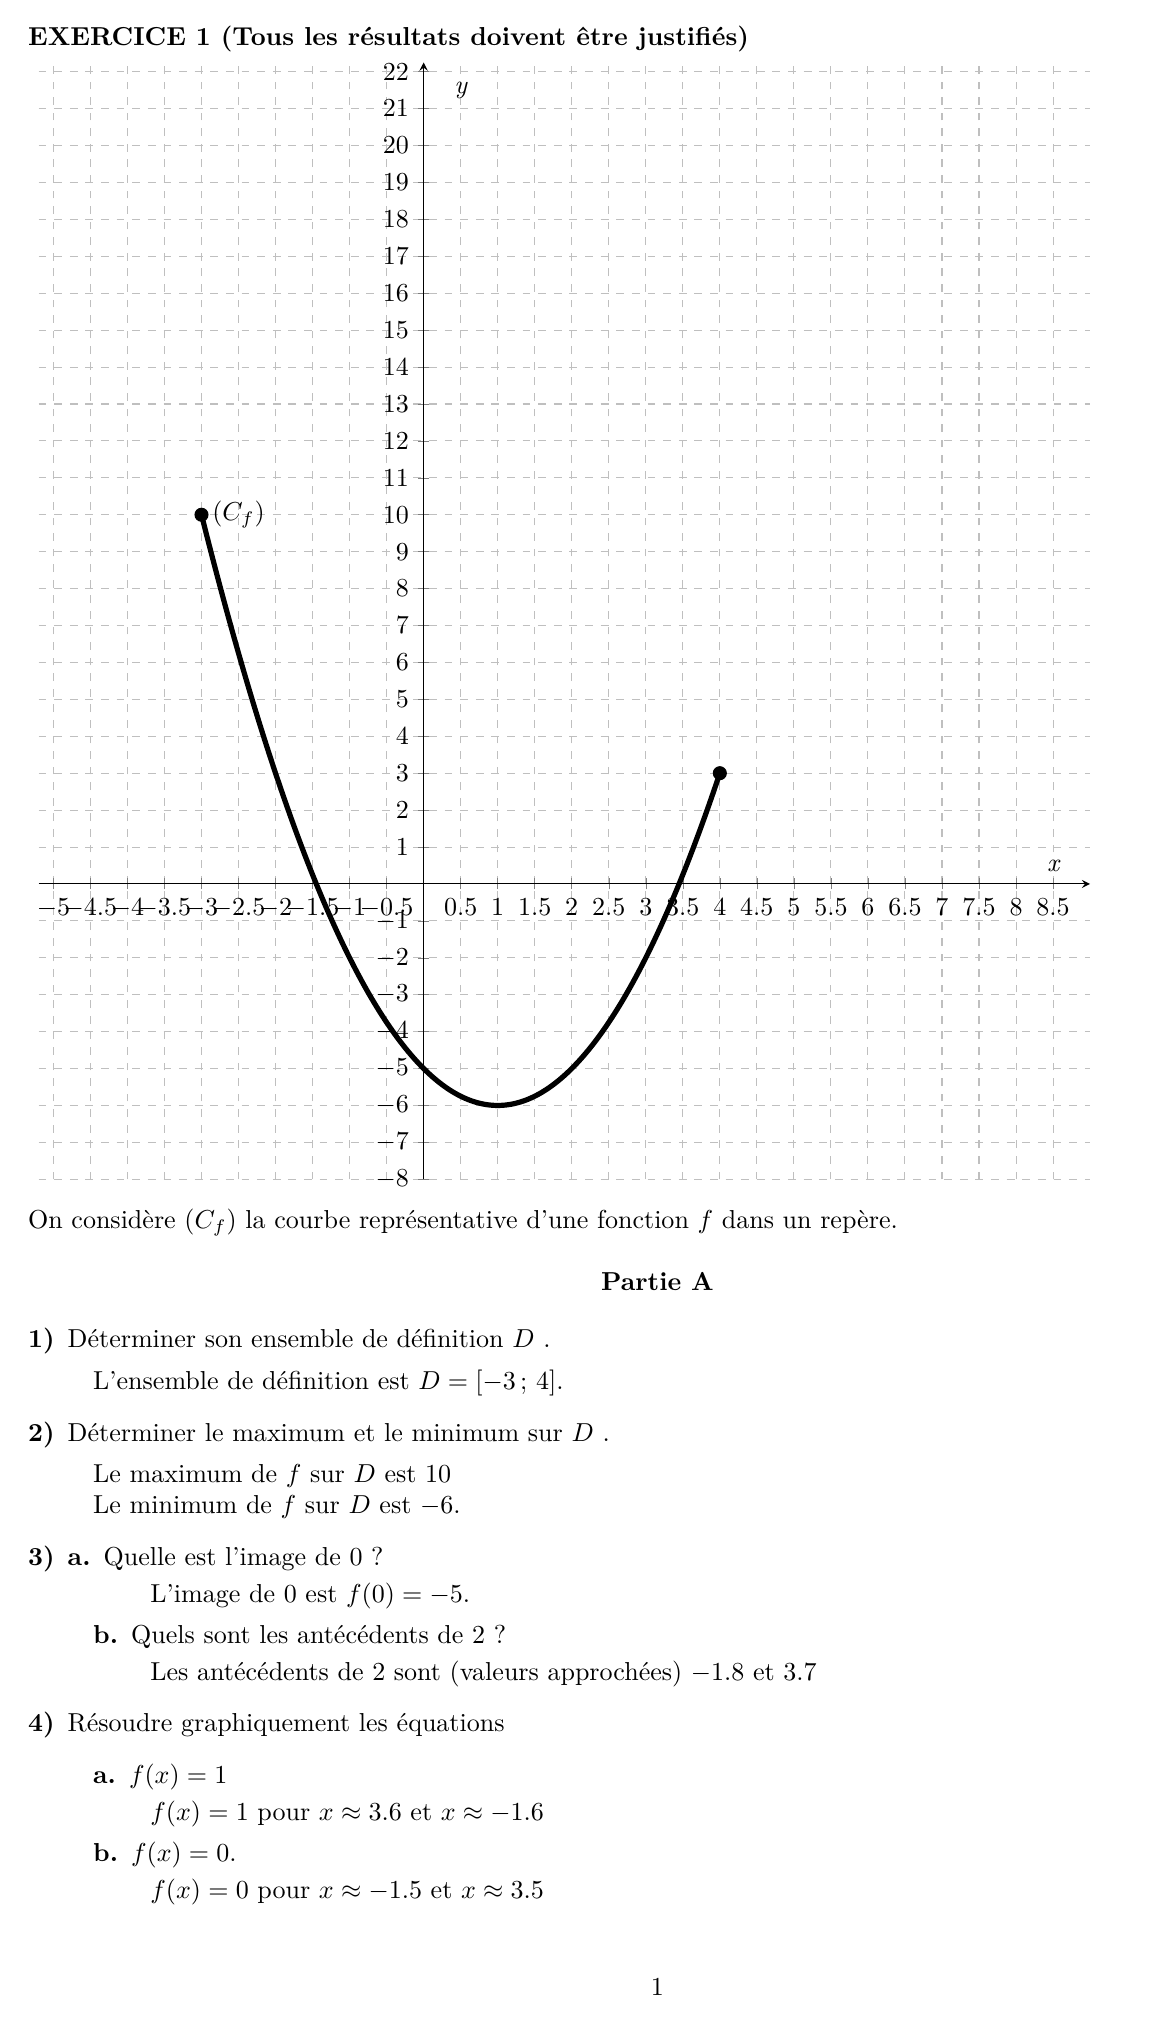
\includegraphics[width=5cm,height=7cm]{./images/creation_exercice_02.png}
 % creation_exercice_02.png: 1166x2018 px, 96dpi, 30.85x53.39 cm, bb=0 0 874 1513
% \caption{1ere page}
% \label{fig:02}
%\end{figure}
&
% \begin{figure}[h]
 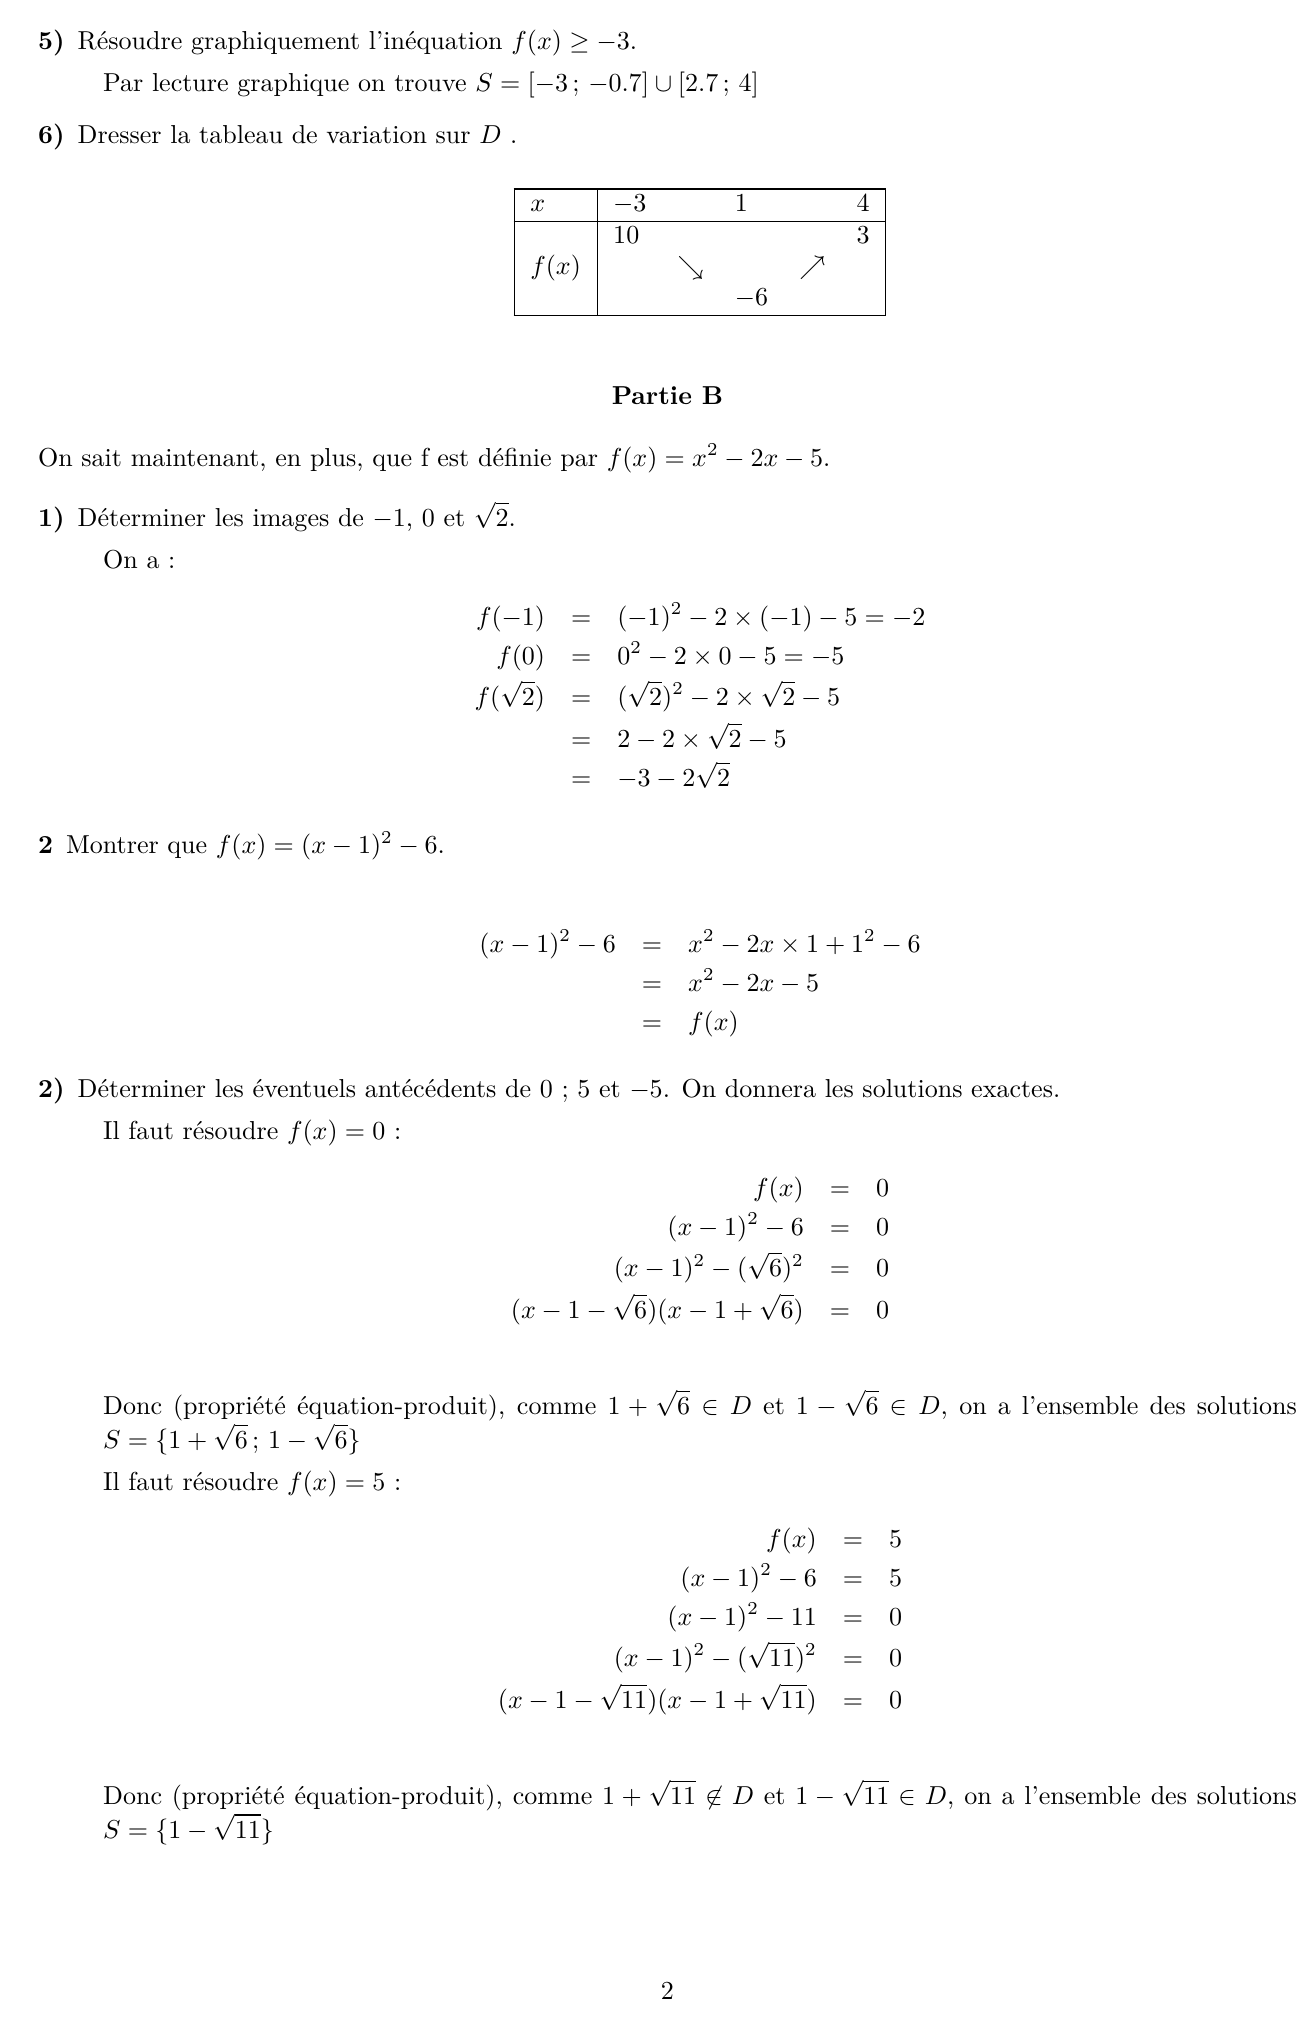
\includegraphics[width=5cm,height=7cm]{./images/creation_exercice_03.png}
 % creation_exercice_02.png: 1166x2018 px, 96dpi, 30.85x53.39 cm, bb=0 0 874 1513
% \caption{2nd page}
% \label{fig:03}
%\end{figure}
\end{tabular}
\end{center}


\begin{dsxl}
L'étape 2 consiste à insérer les \index[dsxlindex]{balises $\%E>$ (début énoncé)  $\%E<$ (fin énoncé),  $\%C>$ (début corrigé)  $\%C<$ (fin corrigé)}, dans la zone de texte à gauche pour indiquer au programme le début et la fin de l'énoncé. 
\end{dsxl}

Le texte avec les balises devient : 
\begin{verbatim}
 On considère $(C_f)$ la courbe représentative d'une fonction $f $ dans un repère.

\bigskip
\centerline{\bf Partie A}

\begin{description}
\item[1)] 
%E>
Déterminer son ensemble de définition $D$ .
%E<
%C>
L'ensemble de définition est $D = [-3\,;\,4]$. 
%C<
\end{verbatim}

Si on clique sur le bouton \fbox{WRAP UP!}, on obtient à droite le text suivant : 

\begin{verbatim}
 On considère $(C_f)$ la courbe représentative d'une fonction $f $ dans un repère.

\bigskip
\centerline{\bf Partie A}

\begin{description}
\item[1)] 
\enonce{ %début énoncé 

Déterminer son ensemble de définition $D$ .
} % fin énoncé 

\correction{ %début correction 

L'ensemble de définition est $D = [-3\,;\,4]$. 
} % fin correction 
\end{verbatim}

\begin{remarque}

\begin{enumerate}
 \item  Les balises commencent toutes par \%. Elles sont donc invisible lors de la compilation de \\
 {\bf DSXL\_3\_programme/dsxl\_tex\_exercice/latex\_wrapper\_in\_full/dsxl\_text\_latex\_wrapper\_in.tex}
 \item Attention à ne par mettre des balises qui enjambent des environnements ou qui contiennent des commandes comme $\backslash$item. 
\end{enumerate}


\end{remarque}

La compilation du fichier 

 {\bf DSXL\_3\_programme/dsxl\_tex\_exercice/latex\_wrapper\_in\_full/dsxl\_text\_latex\_wrapper\_out.tex}
 
 donne : 

 \begin{center}
 \begin{tabular}{ccc}
 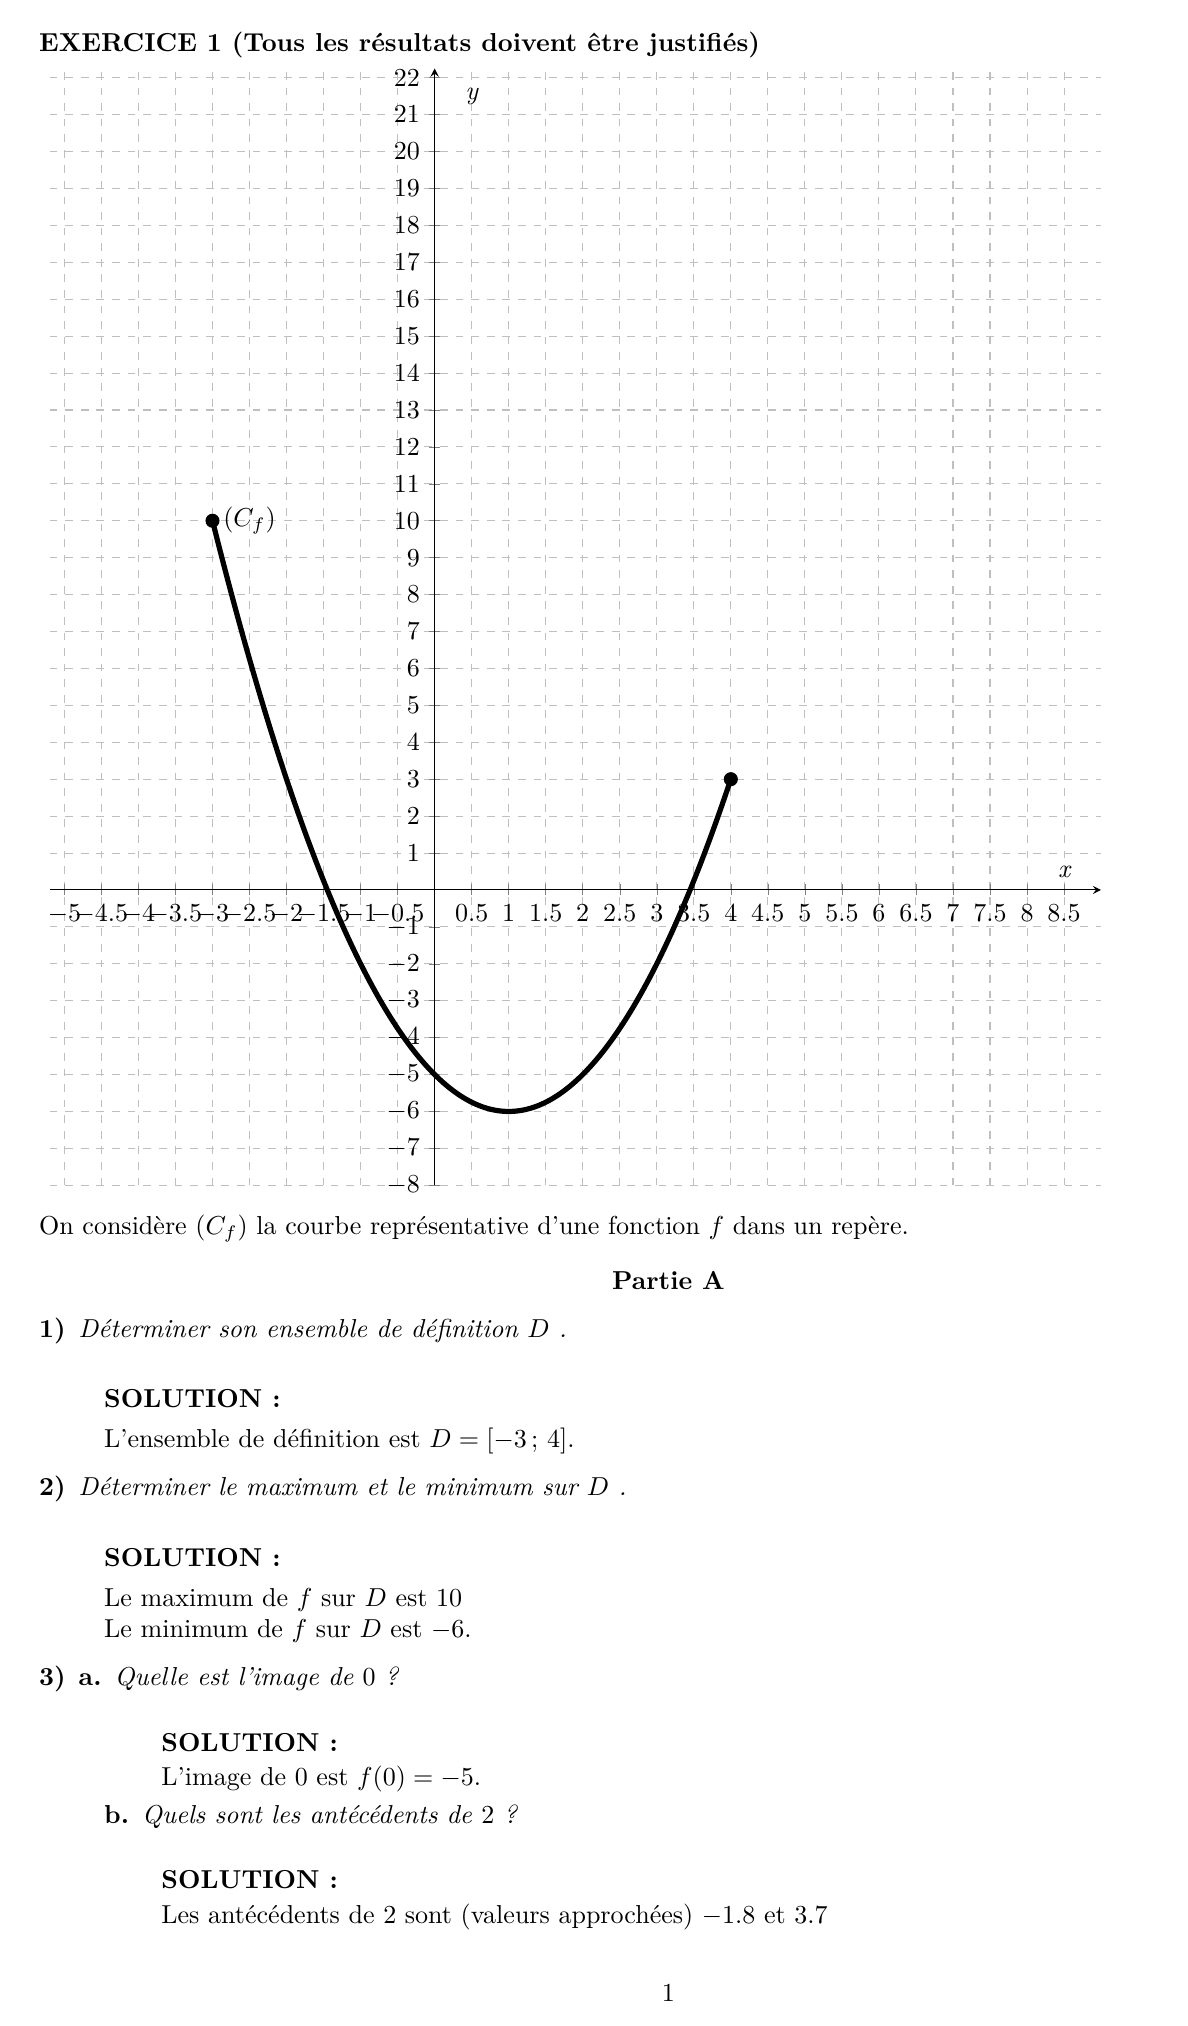
\includegraphics[width=5cm,height=7cm]{./images/creation_exercice_04.png}
&
 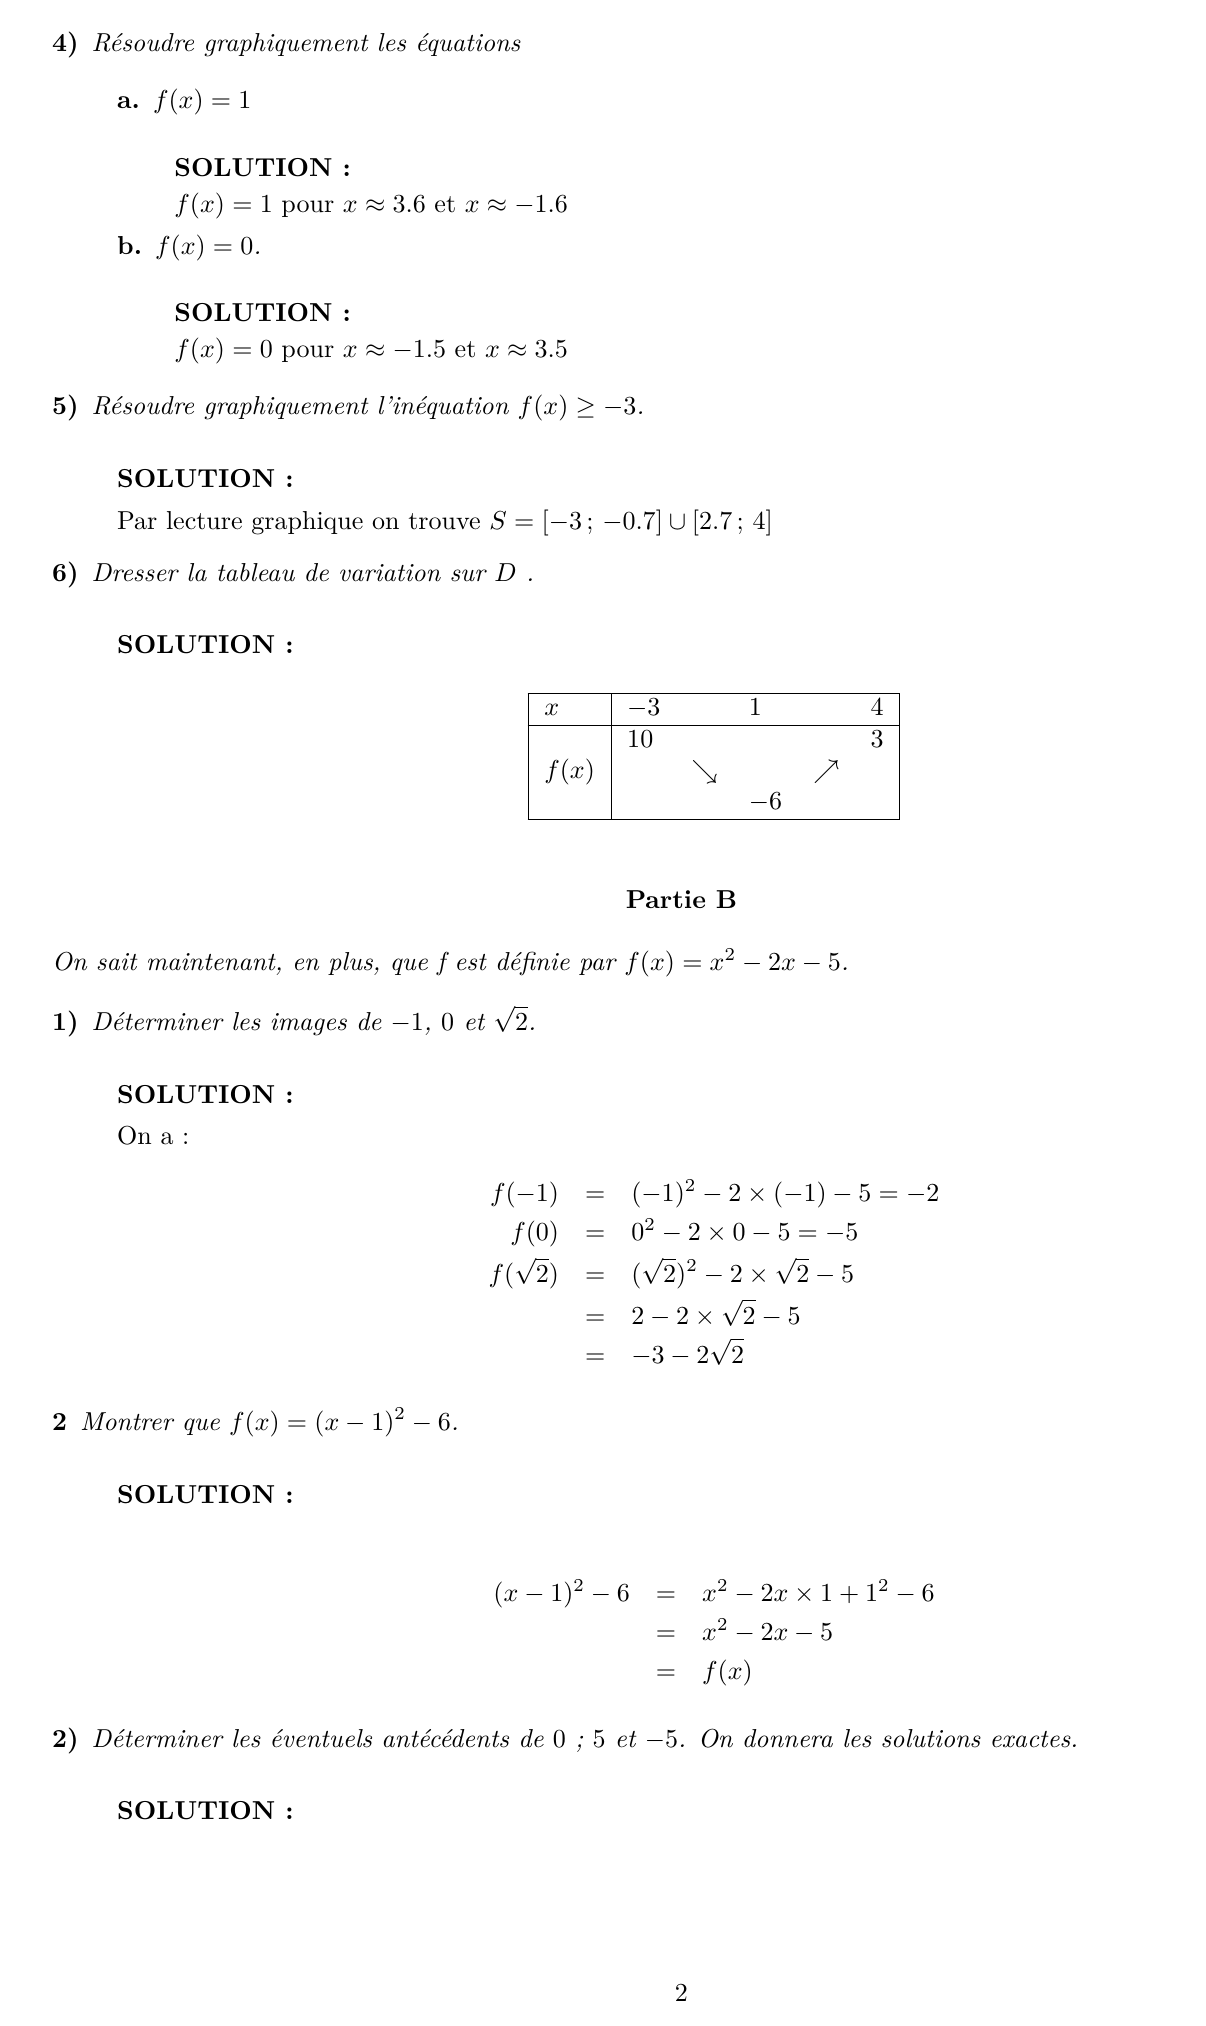
\includegraphics[width=5cm,height=7cm]{./images/creation_exercice_05.png}
 &
 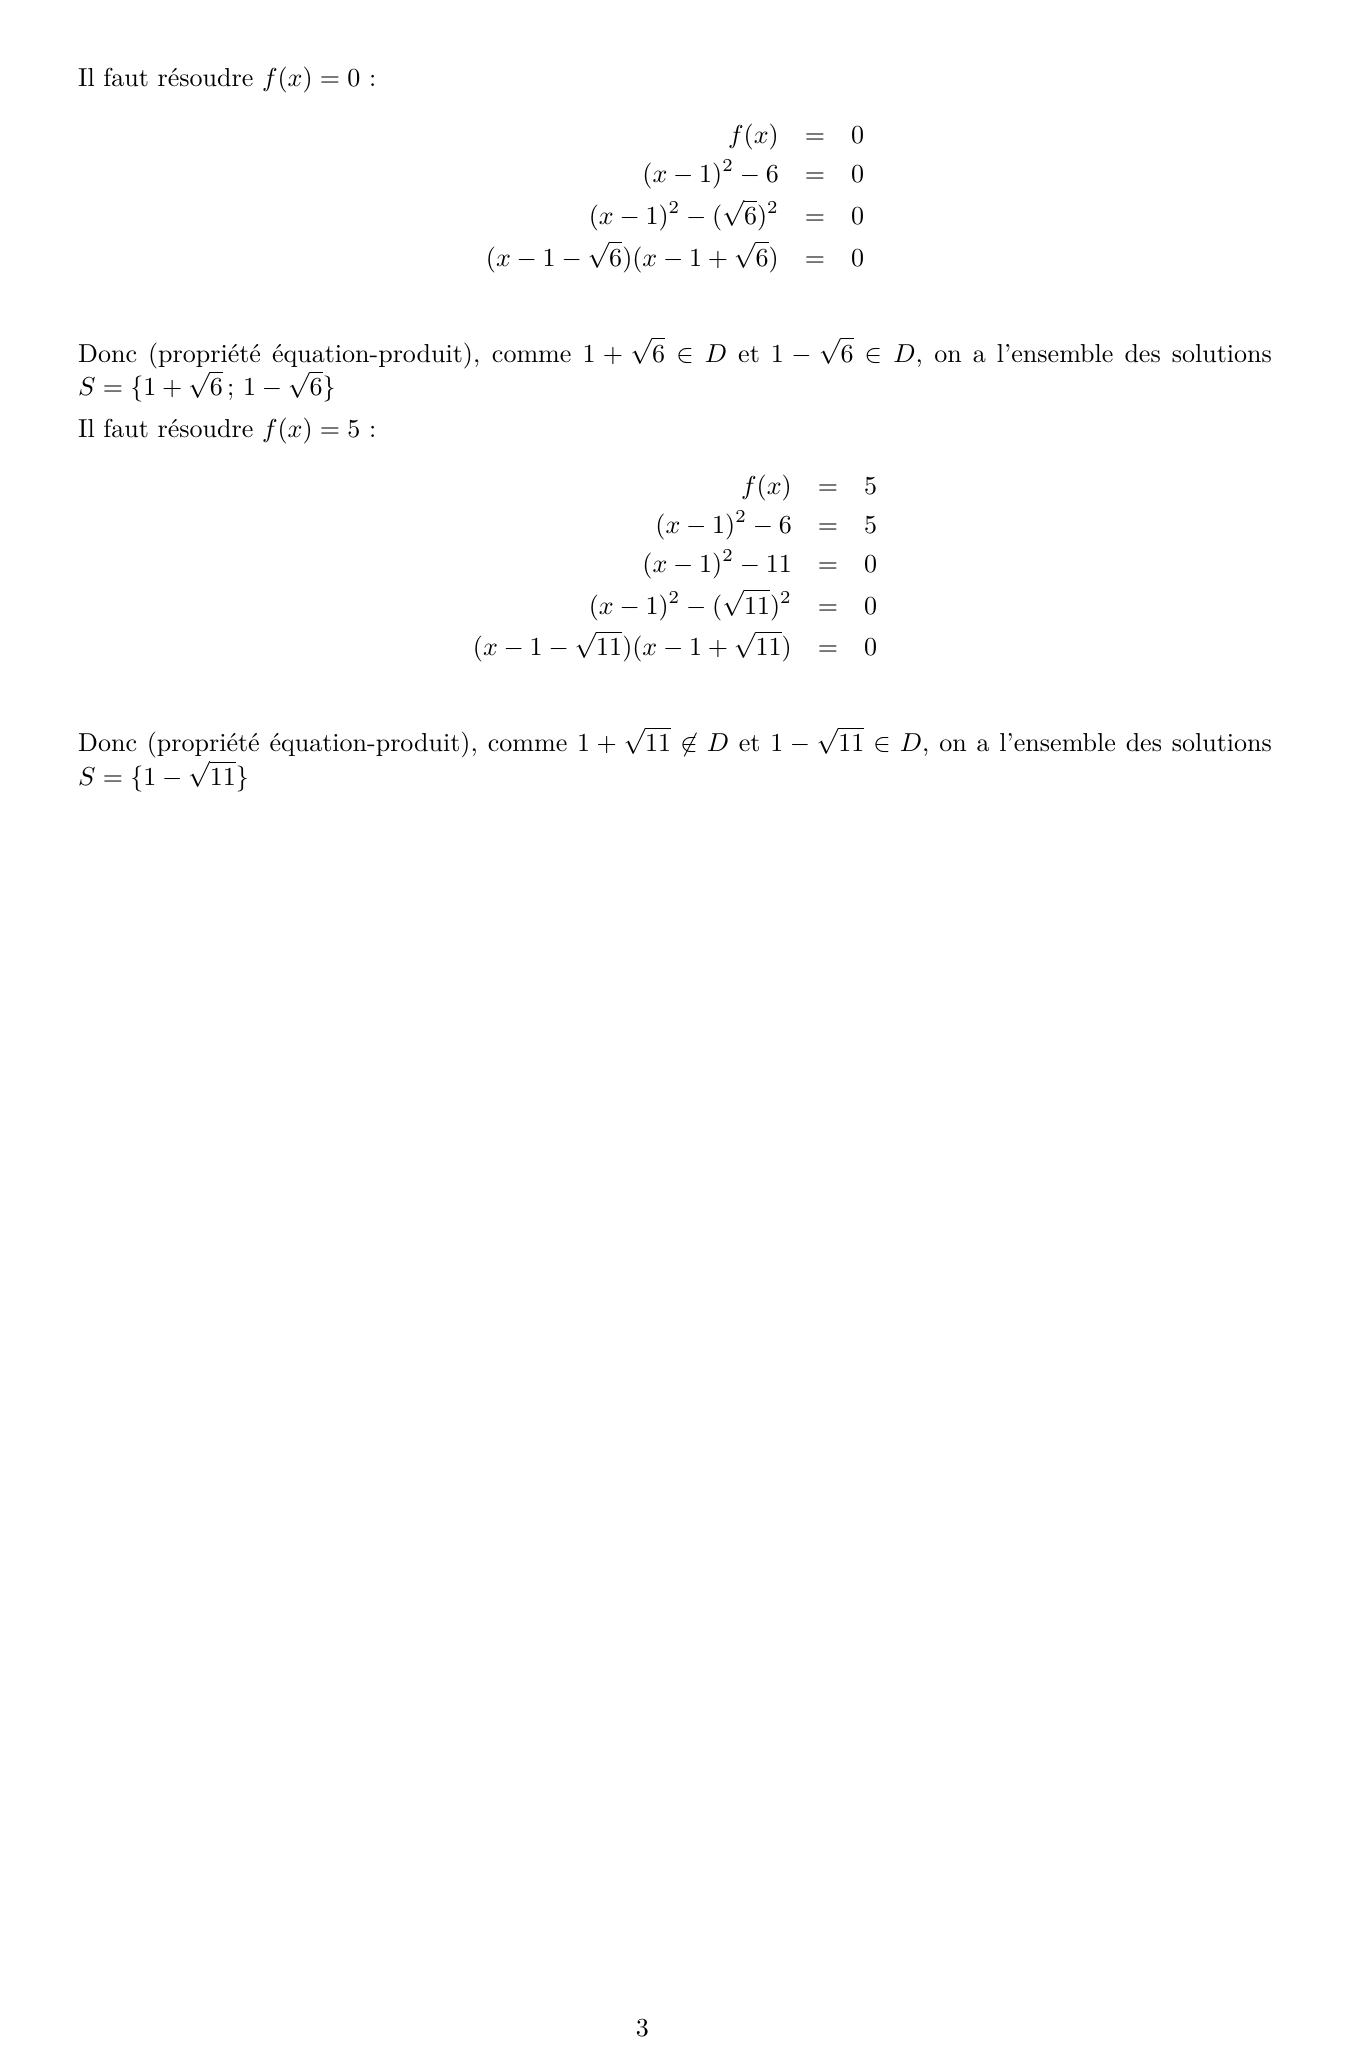
\includegraphics[width=5cm,height=7cm]{./images/creation_exercice_06.png}
\end{tabular}
\end{center}

\begin{dsxl}
 Le réglage entre le \index[dsxlindex]{mode E}mode E = Enoncé et \index[dsxlindex]{mode C}mode C = Correction se fait au niveau des lignes ci-dessous.
 Voici le mode correction qui a donné le texte ci-dessus : 
 \begin{verbatim}
% *********************************************************************
% MODIFIER LA LIGNE SELON LE MODE VOULU : **********************
\newcommand{\EnonceCorrection}{C}	% E = mode énoncé   C = mode correction 
% **********************************************************************
 \end{verbatim}

Pour avoir le mode énoncé : \\
 \begin{verbatim}
% *********************************************************************
% MODIFIER LA LIGNE SELON LE MODE VOULU : **********************
\newcommand{\EnonceCorrection}{E}	% E = mode énoncé   C = mode correction 
% **********************************************************************
 \end{verbatim}
Le texte compilé donne le fichier pdf suivant : 

 \begin{center}
 \begin{tabular}{cc}
 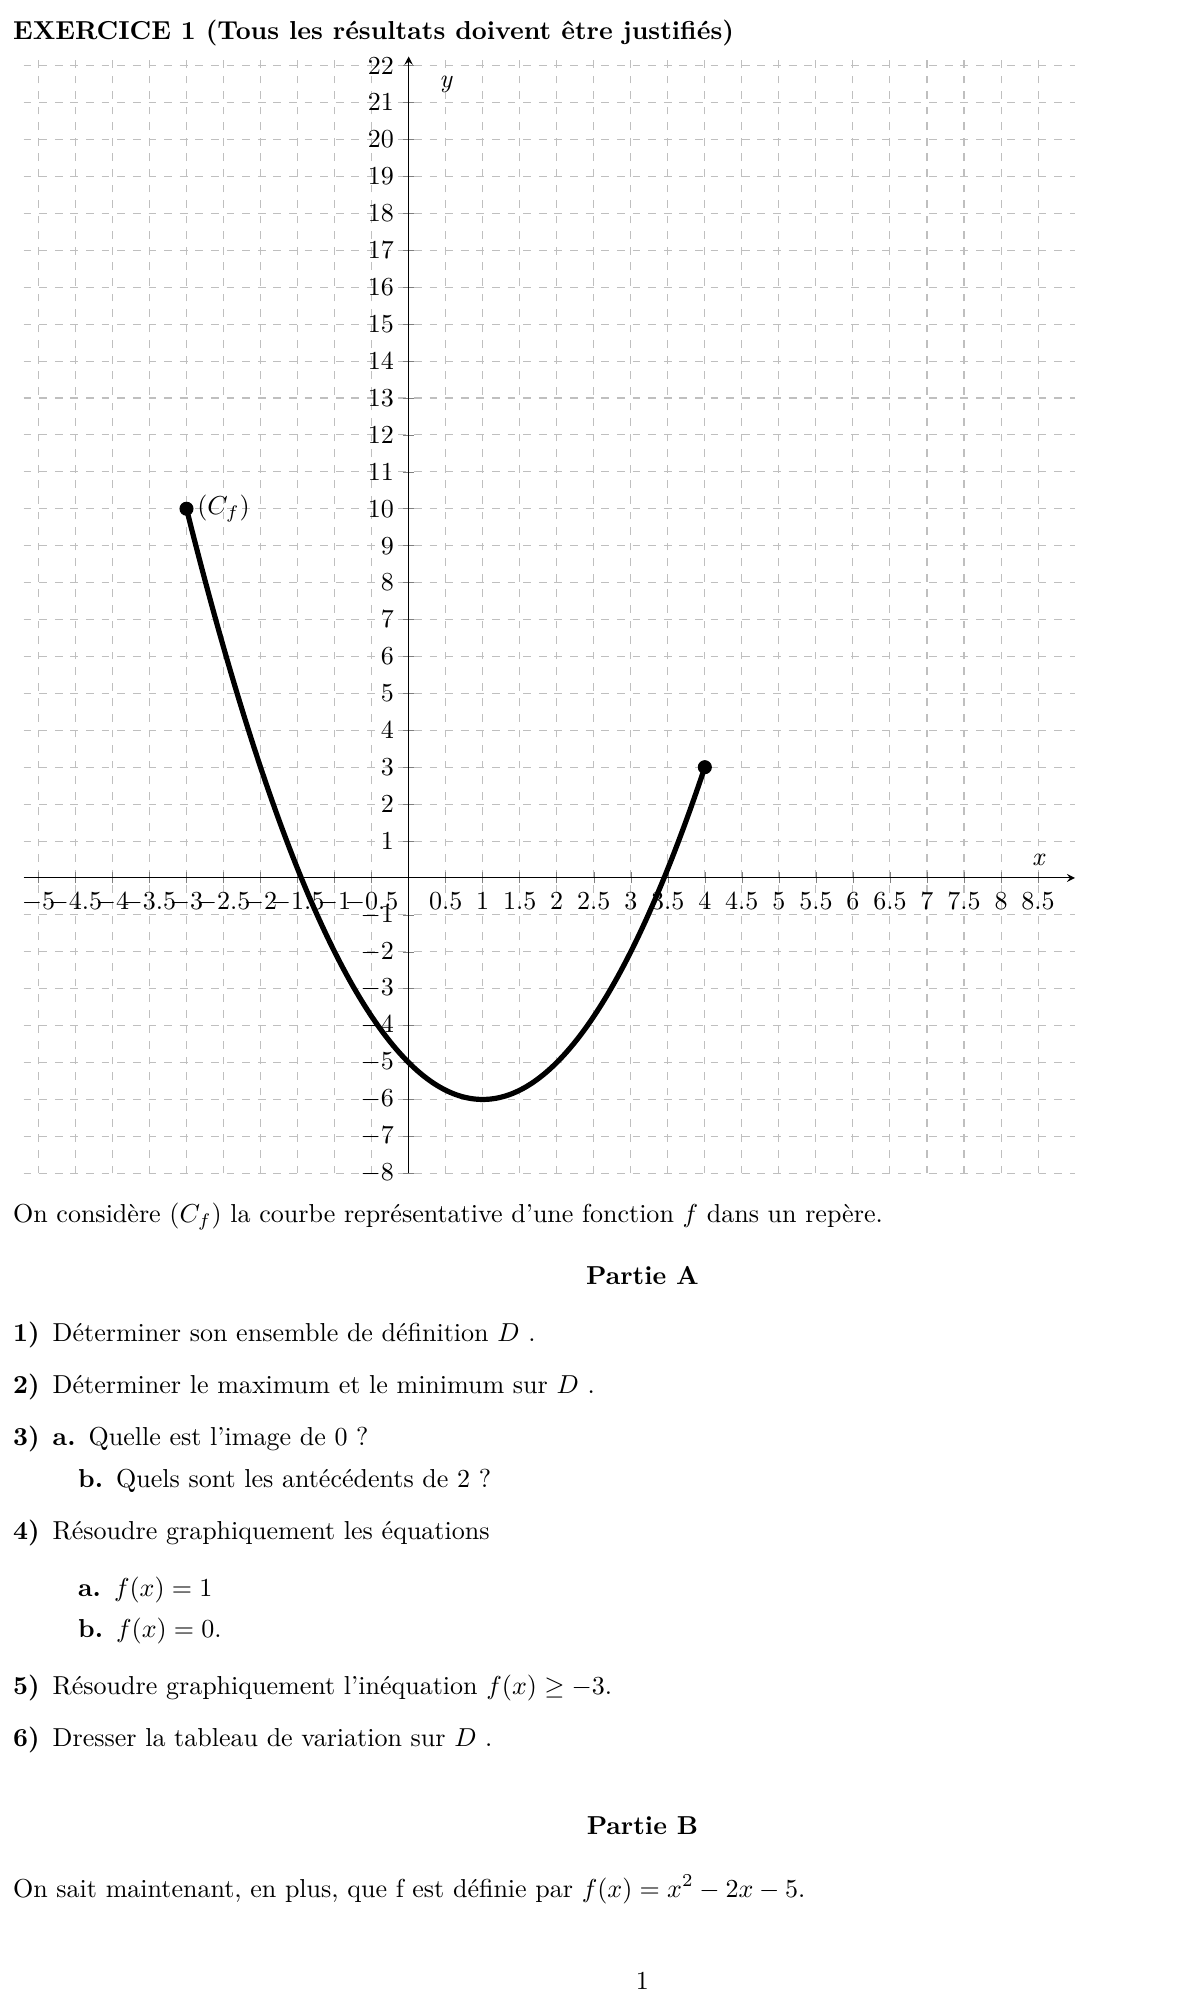
\includegraphics[width=7cm,height=10cm]{./images/creation_exercice_07.png}
&
 
\includegraphics[width=7cm,height=10cm]{./images/creation_exercice_08.png}
\end{tabular}
\end{center}
On constate que seul l'énoncé est présent. 
\end{dsxl}


\subsection{Etape 3 : Définir le barème des questions}

\begin{dsxl}
 Selon le devoir, un exercice va avoir un nombre de points variable. C'est pourquoi on indiquera le poids de la question en pourcentage. 
Le bouton bouton \fbox{$\backslash$poids$\{\}$\% en pourcentage} \index[dsxlindex]{bouton \fbox{$\backslash$poids$\{\}$\% en pourcentage}} permet cela. 
\end{dsxl}

La \index[dsxlindex]{convention barème} suivante sera utilisée dans les exercices : 
\begin{dsxl}
 La commande Latex  \fbox{$\backslash$poids$\{\}$\% en pourcentage} ne sera inséré qu'entre les balises corrigés :  $\%C>$ (début corrigé)  $\%C<$ (fin corrigé)
\end{dsxl}

Le barème n'est donc visible pour les élèves que dans le mode C (correction). Pour faire apparaître le barème en mode E (énoncé), la commande 
\begin{verbatim}
  \SeulementModeEnonce{\poids{100} }
\end{verbatim}
pourra être inserée maintenant ou plus tard dans l'énoncé.

\begin{dsxl}
 La commande 
 \begin{verbatim}
  \poids{60}
 \end{verbatim}
va, dans un devoir où cet exercice vaudra 10 points, être remplacée par 
 \begin{verbatim}
  \points{6}
 \end{verbatim}
 car $10\times \frac{60}{100} = 6$. 
\end{dsxl}

Après avoir cliqué sur le bouton  \fbox{$\backslash$poids$\{\}$\% en pourcentage}, la compilation de \\
{\bf\small DSXL\_3\_programme/dsxl\_tex\_exercice/latex\_wrapper\_in\_full/dsxl\_text\_latex\_wrapper\_out.tex}
(qui a été modifié) donne en mode E (la commande $\backslash$SeulementModeEnonce{ $\backslash$poids\{100\} a été insérée après $\backslash$EXERCICE )  :
 \begin{center}
 \begin{tabular}{cc}
 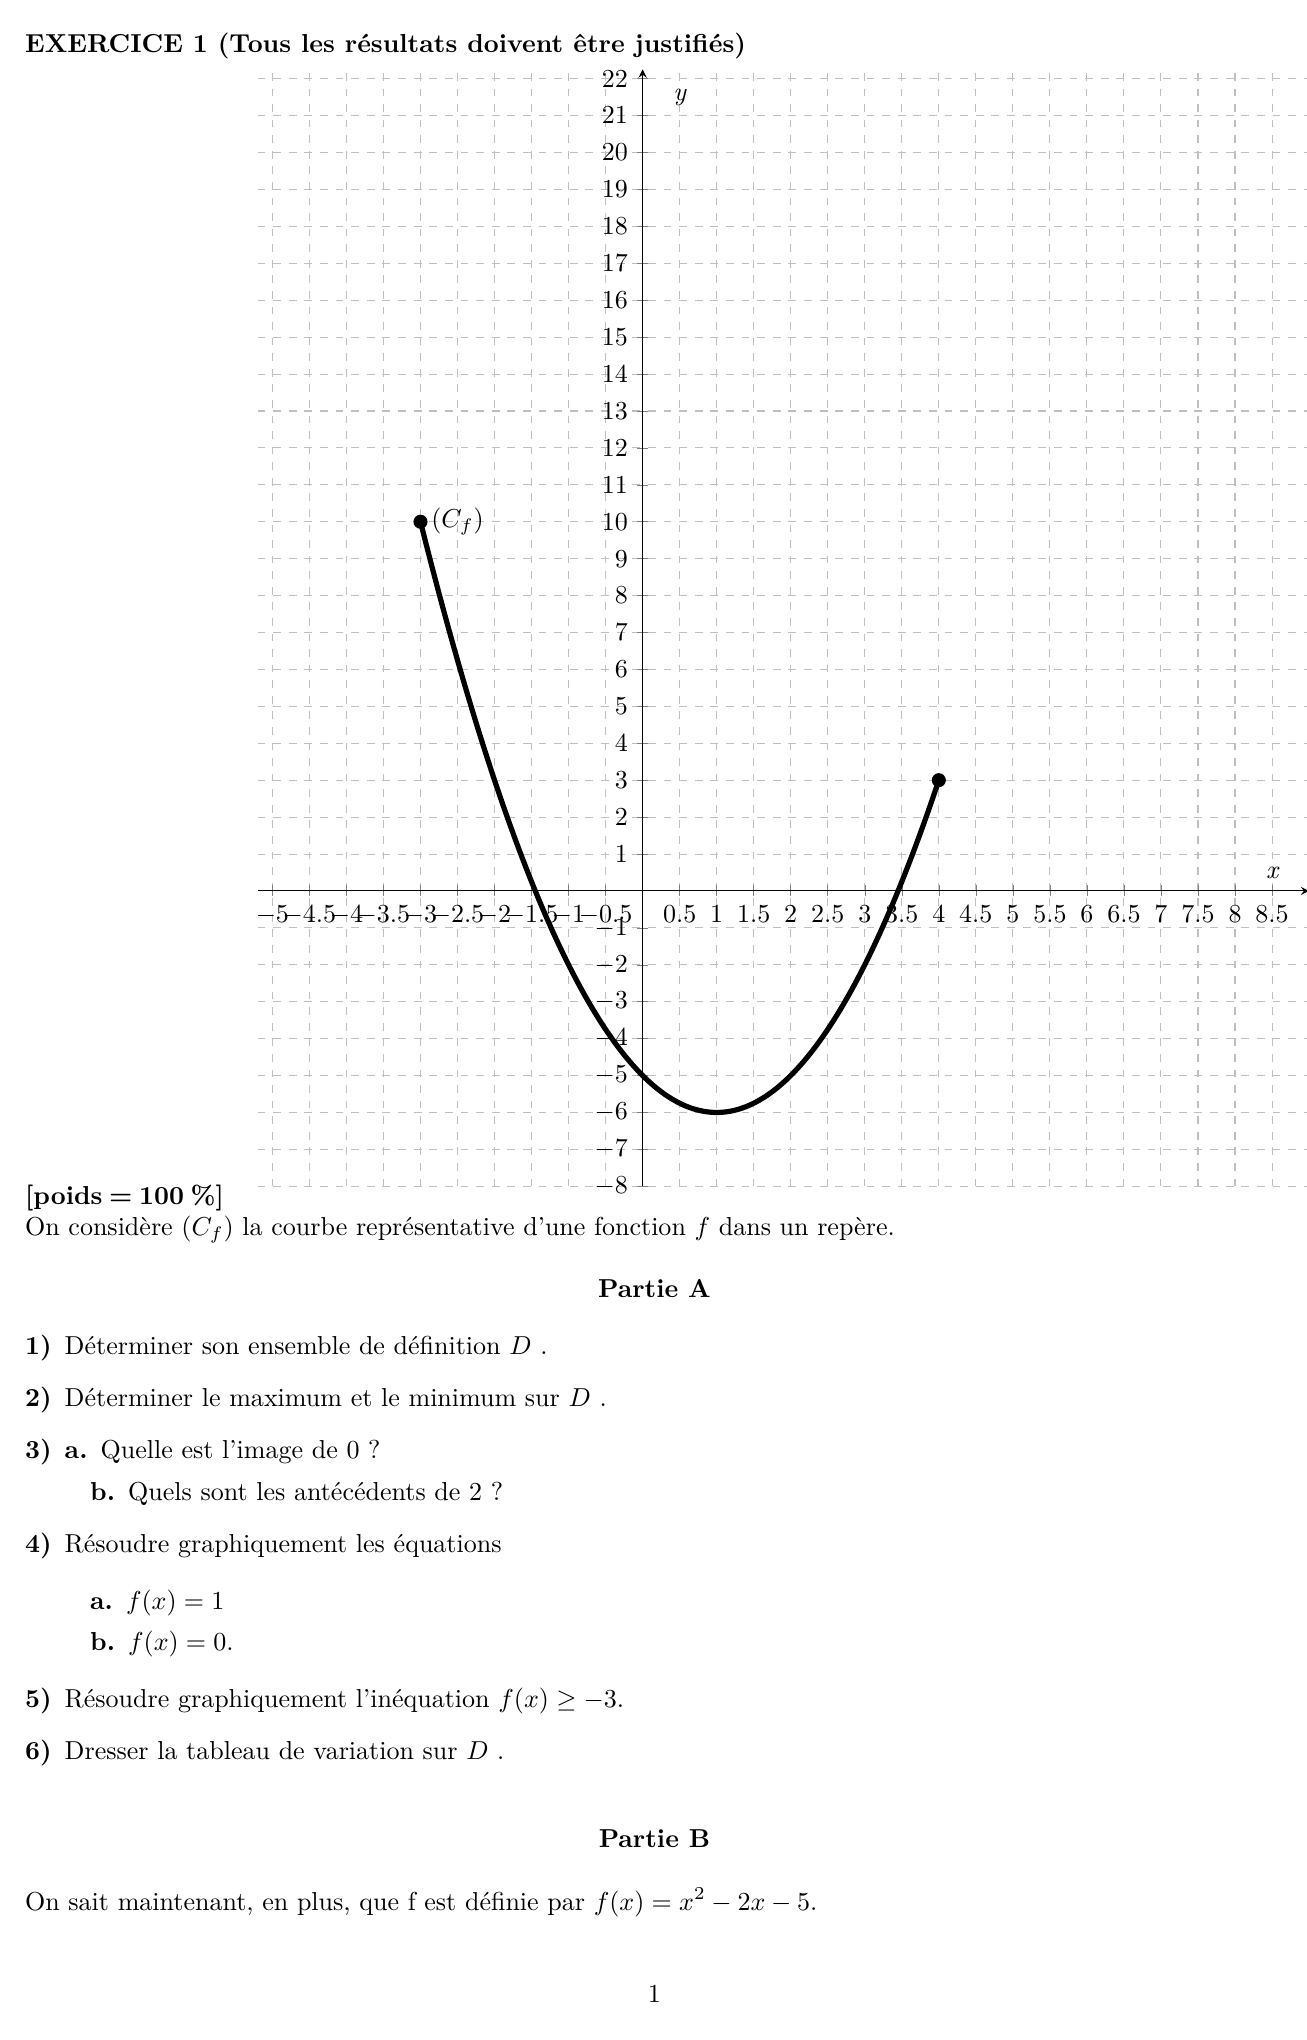
\includegraphics[width=7cm,height=10cm]{./images/creation_exercice_09.png}
&
 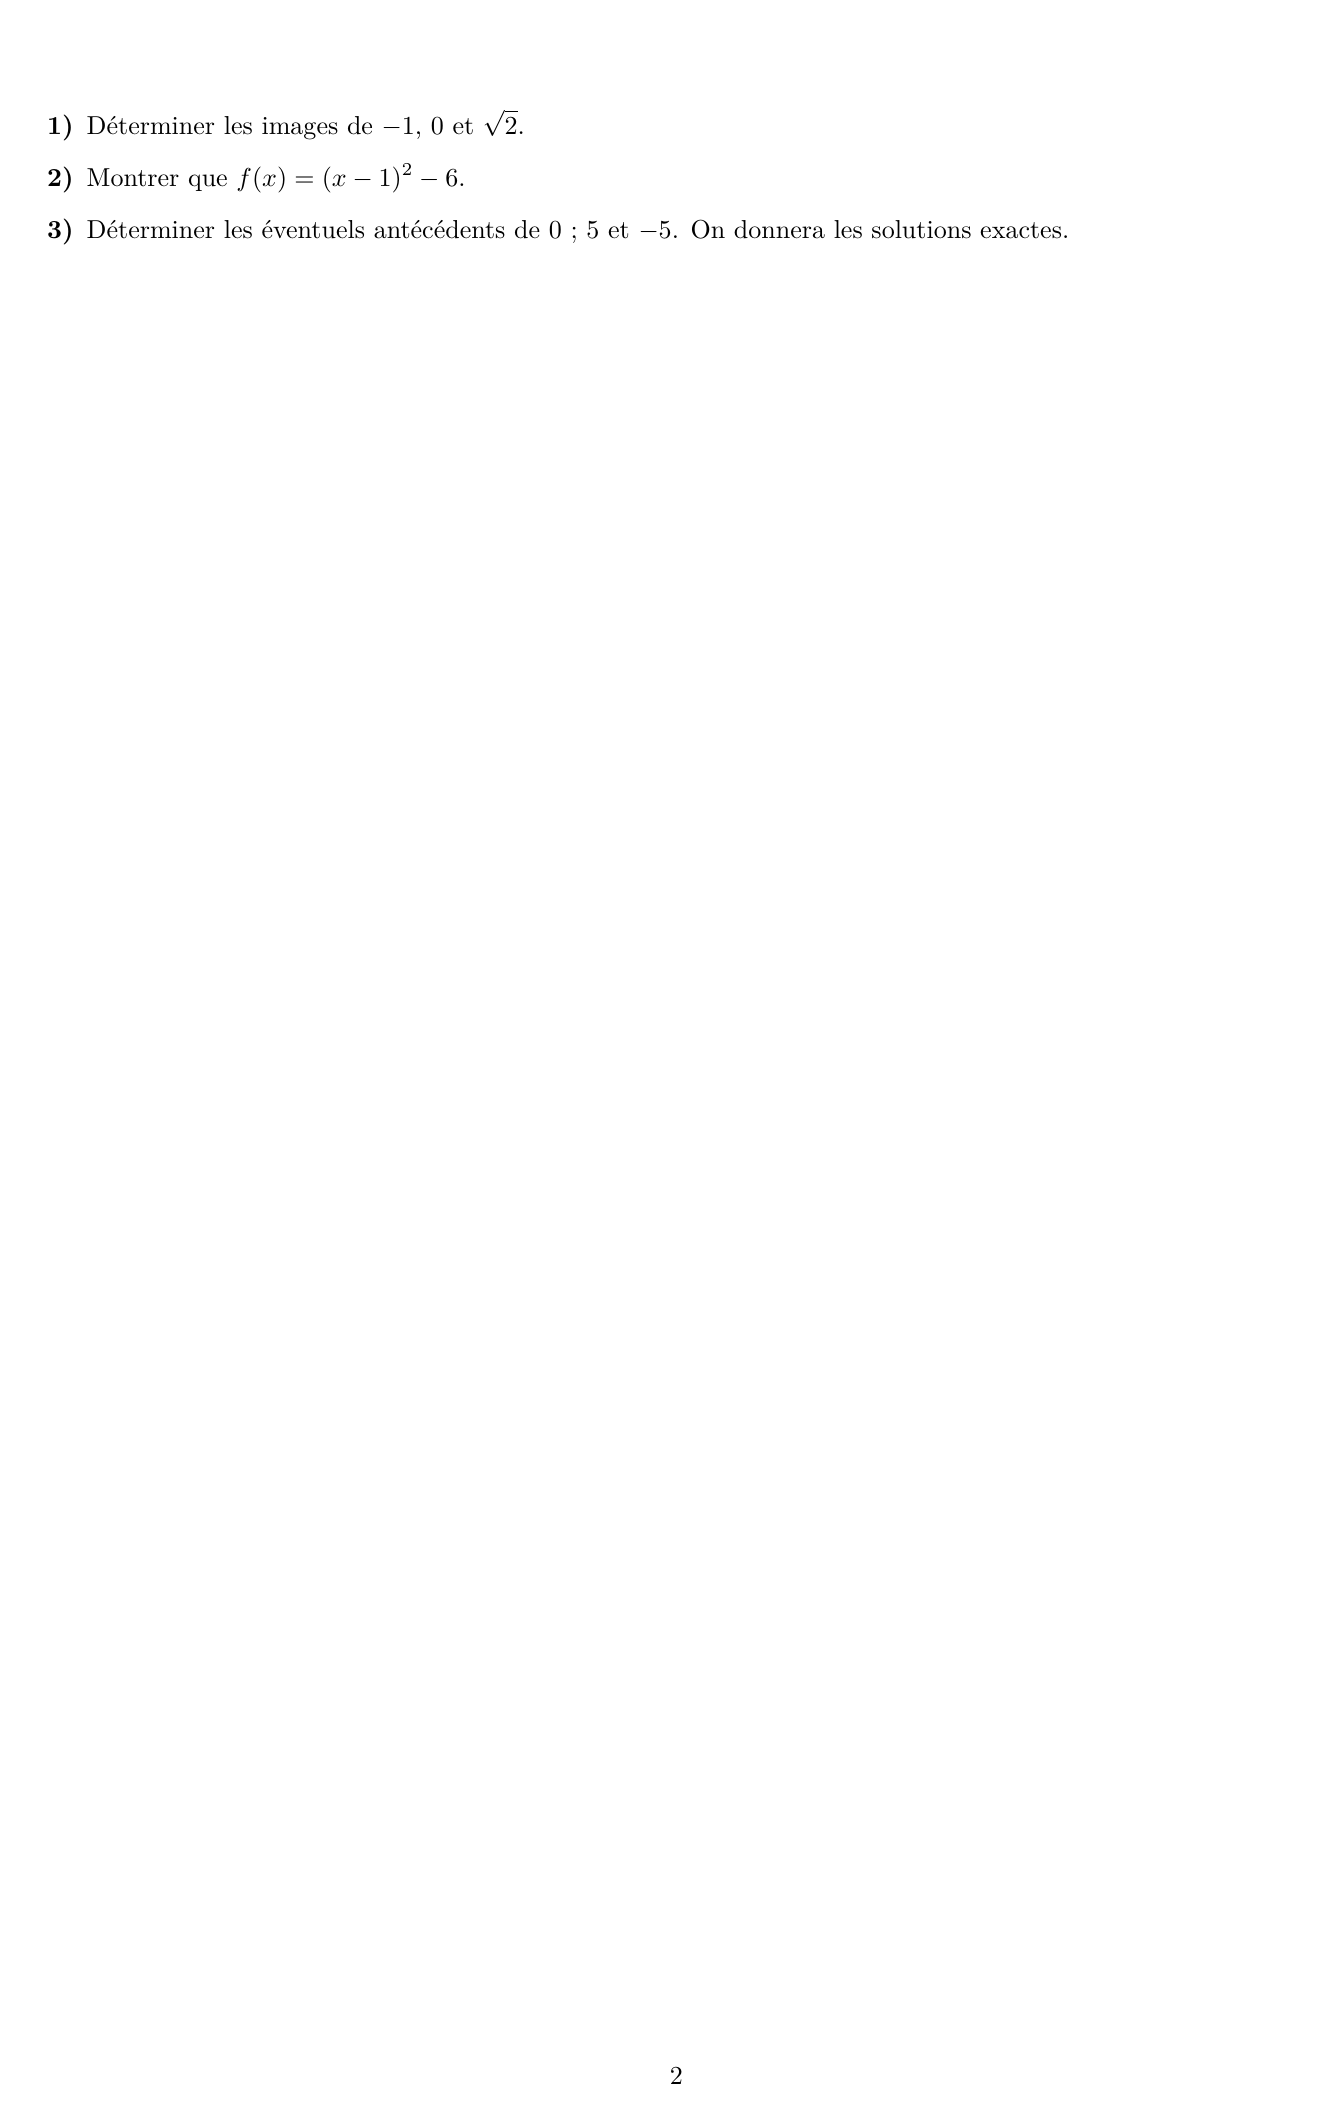
\includegraphics[width=7cm,height=10cm]{./images/creation_exercice_10.png}
\end{tabular}
\end{center}
La compilation de \\
{\bf\small DSXL\_3\_programme/dsxl\_tex\_exercice/latex\_wrapper\_in\_full/dsxl\_text\_latex\_wrapper\_out.tex}
en mode C donne :

 \begin{center}
 \begin{tabular}{ccc}
 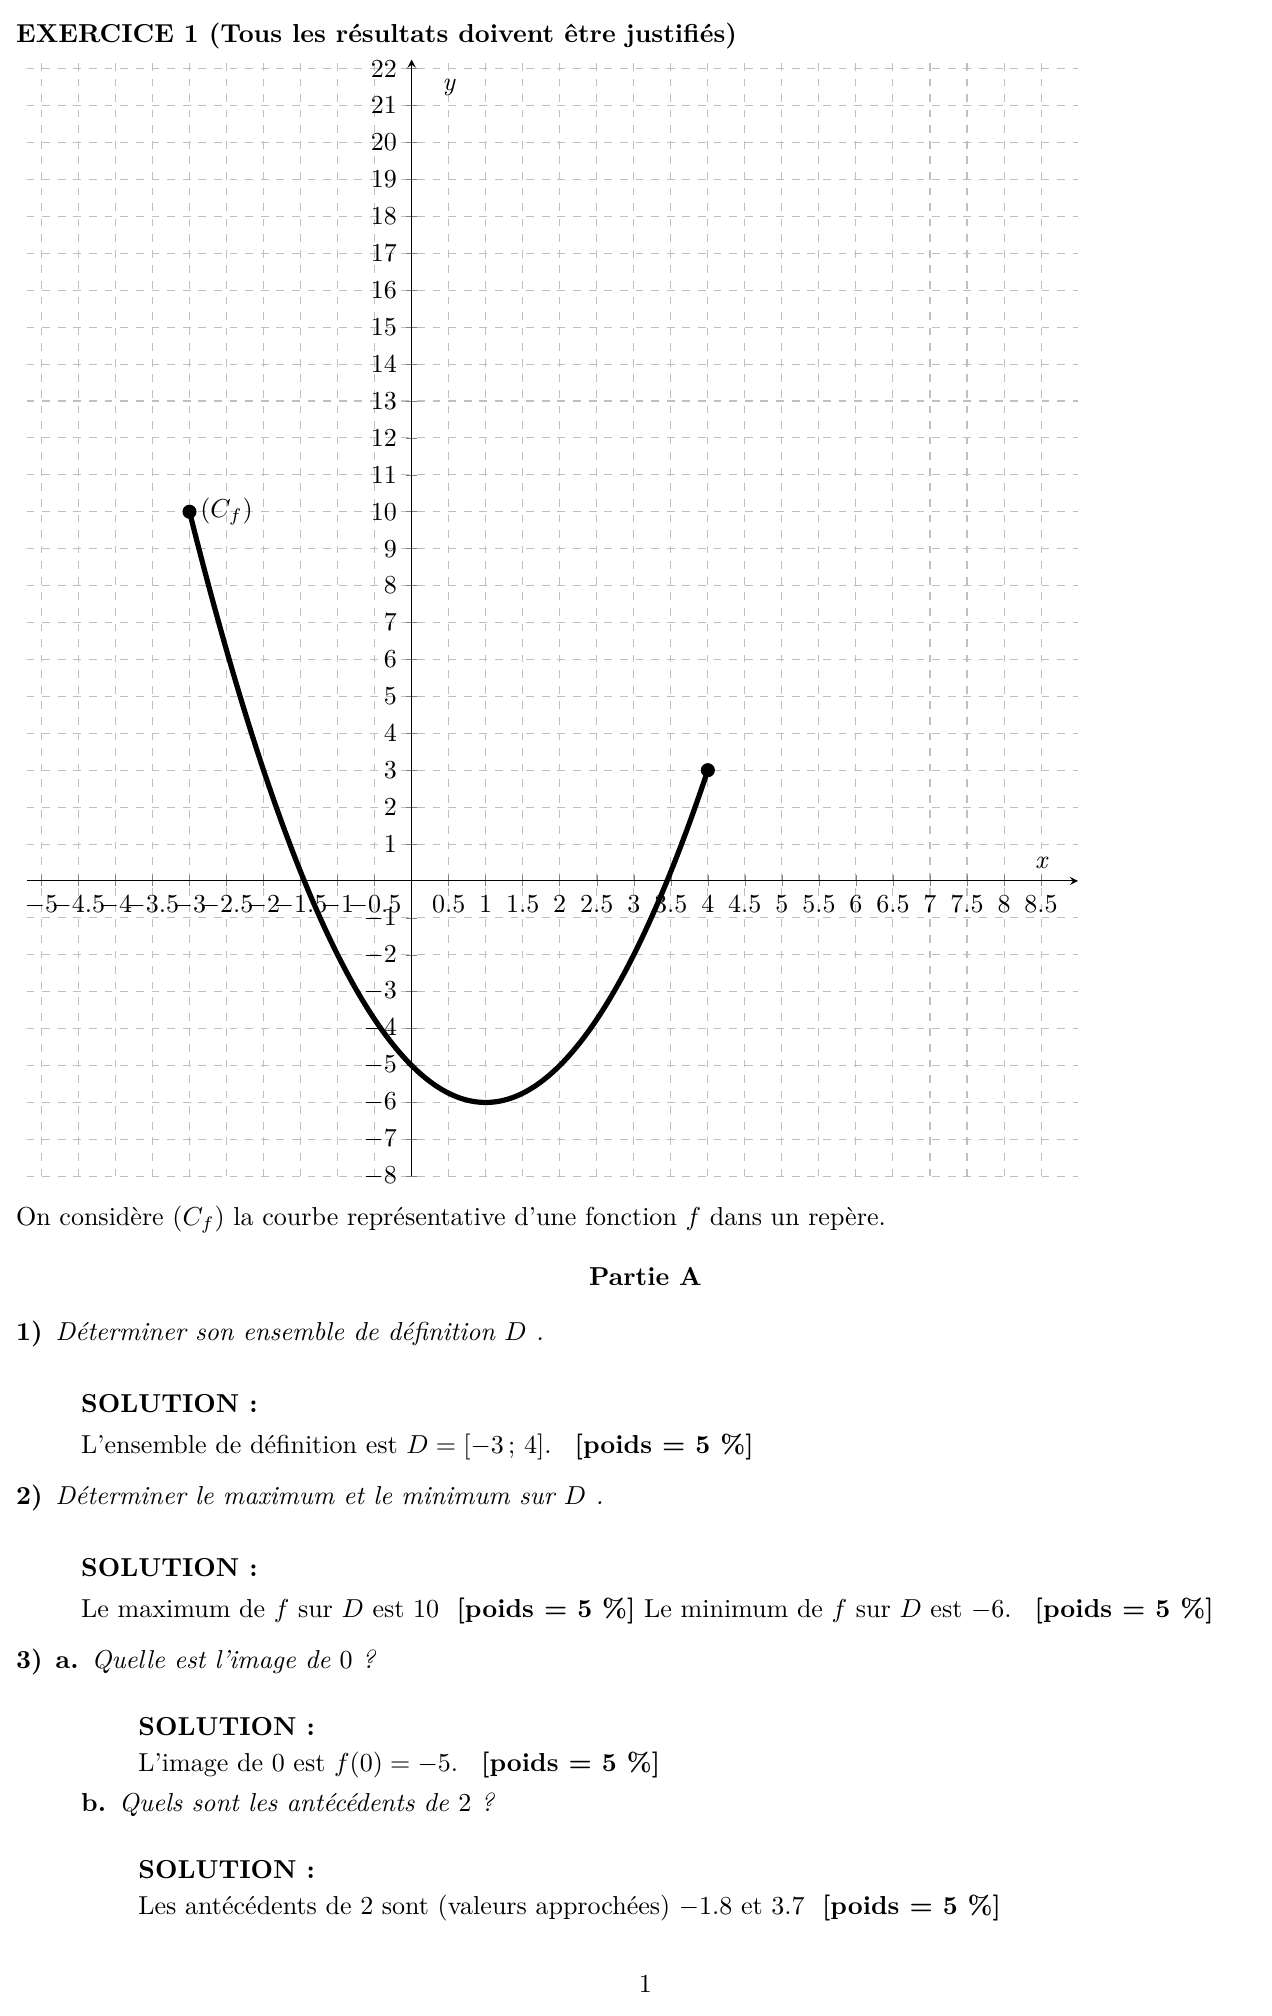
\includegraphics[width=5cm,height=7cm]{./images/creation_exercice_11.png}
&
 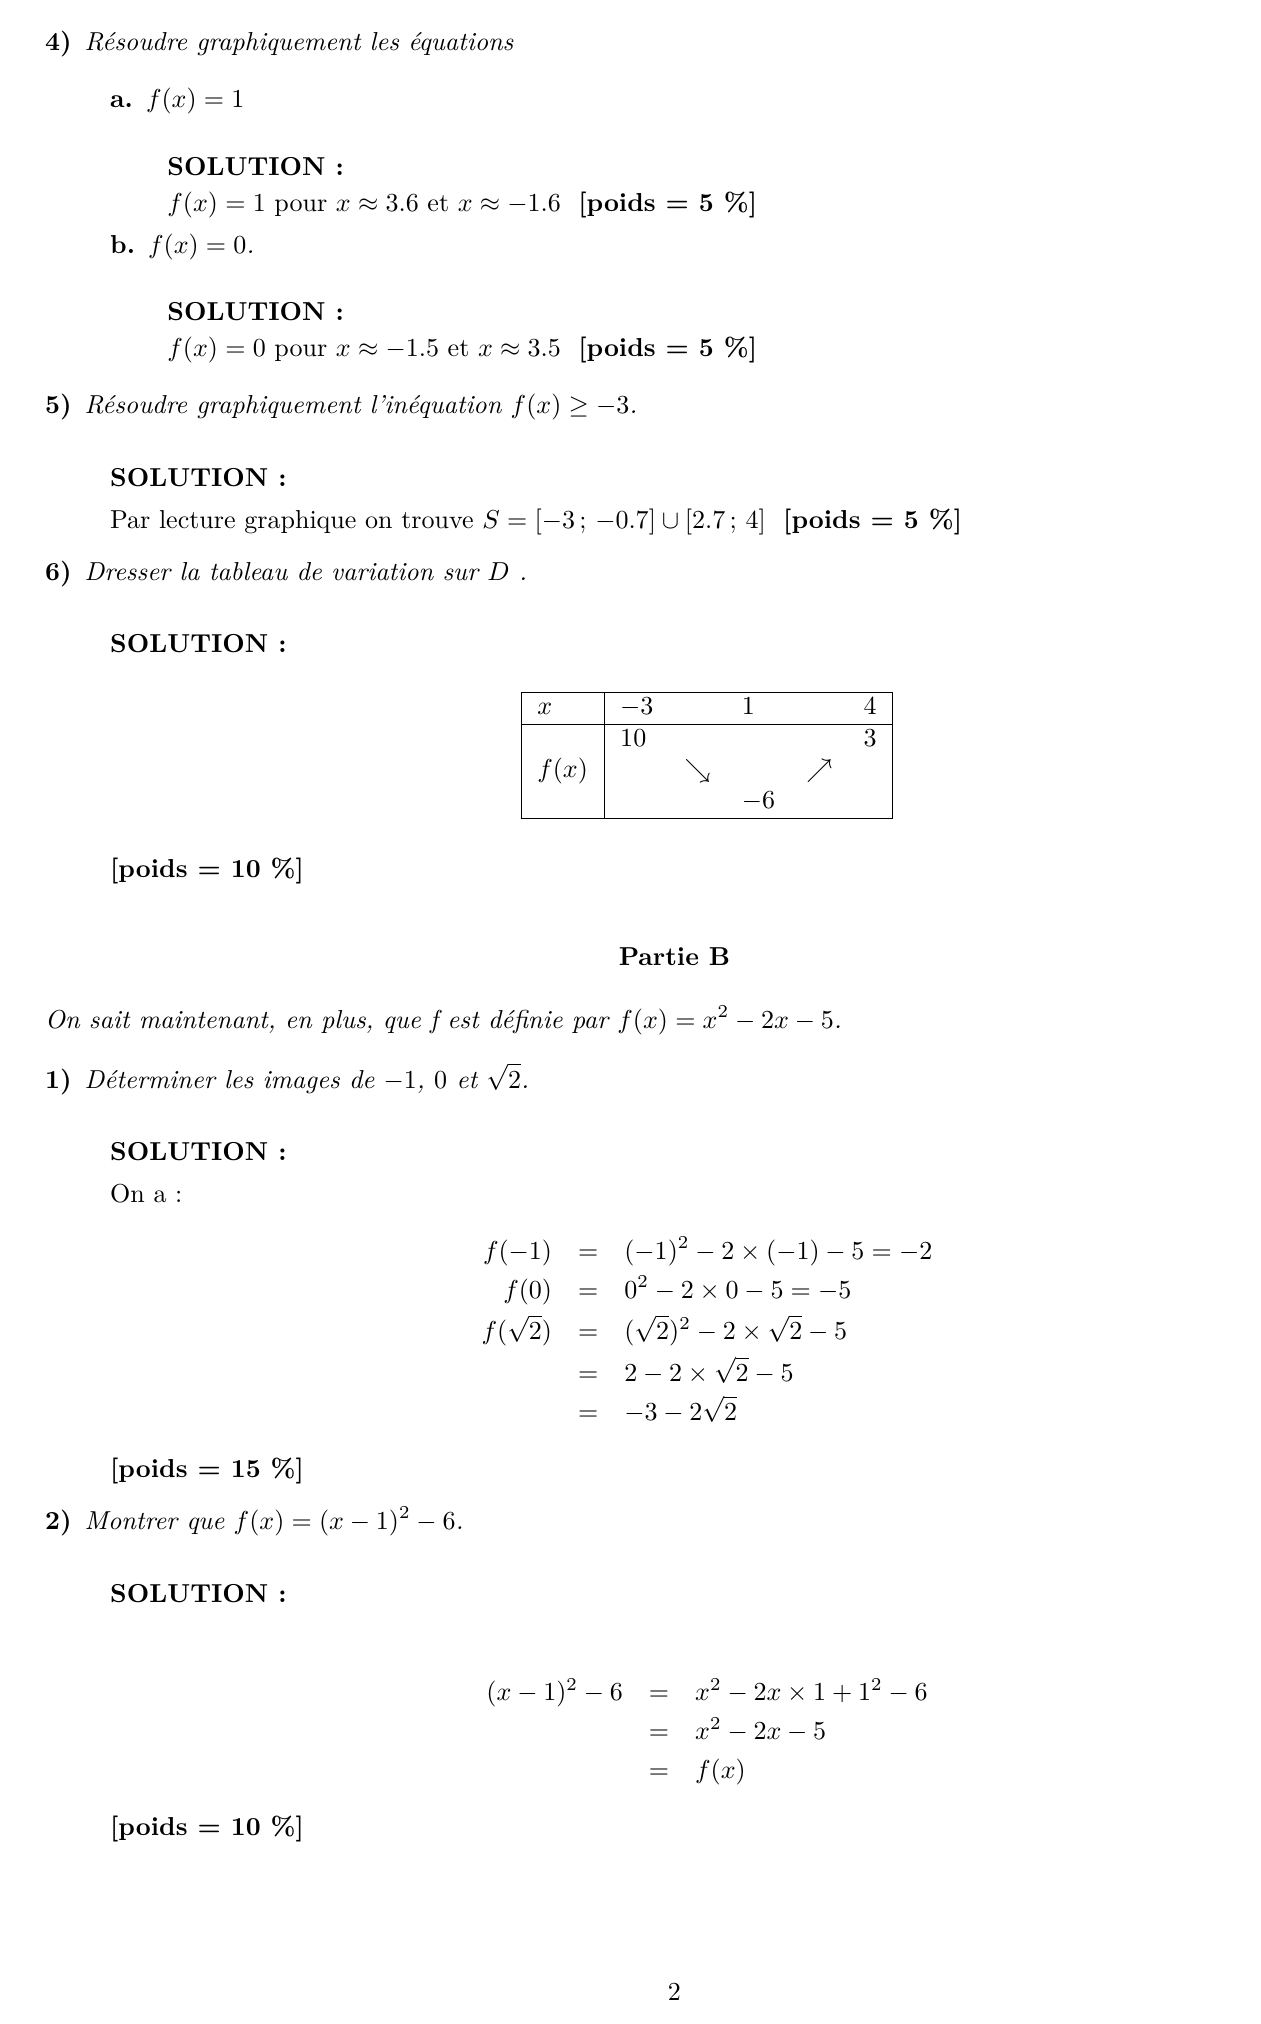
\includegraphics[width=5cm,height=7cm]{./images/creation_exercice_12.png}
 &
 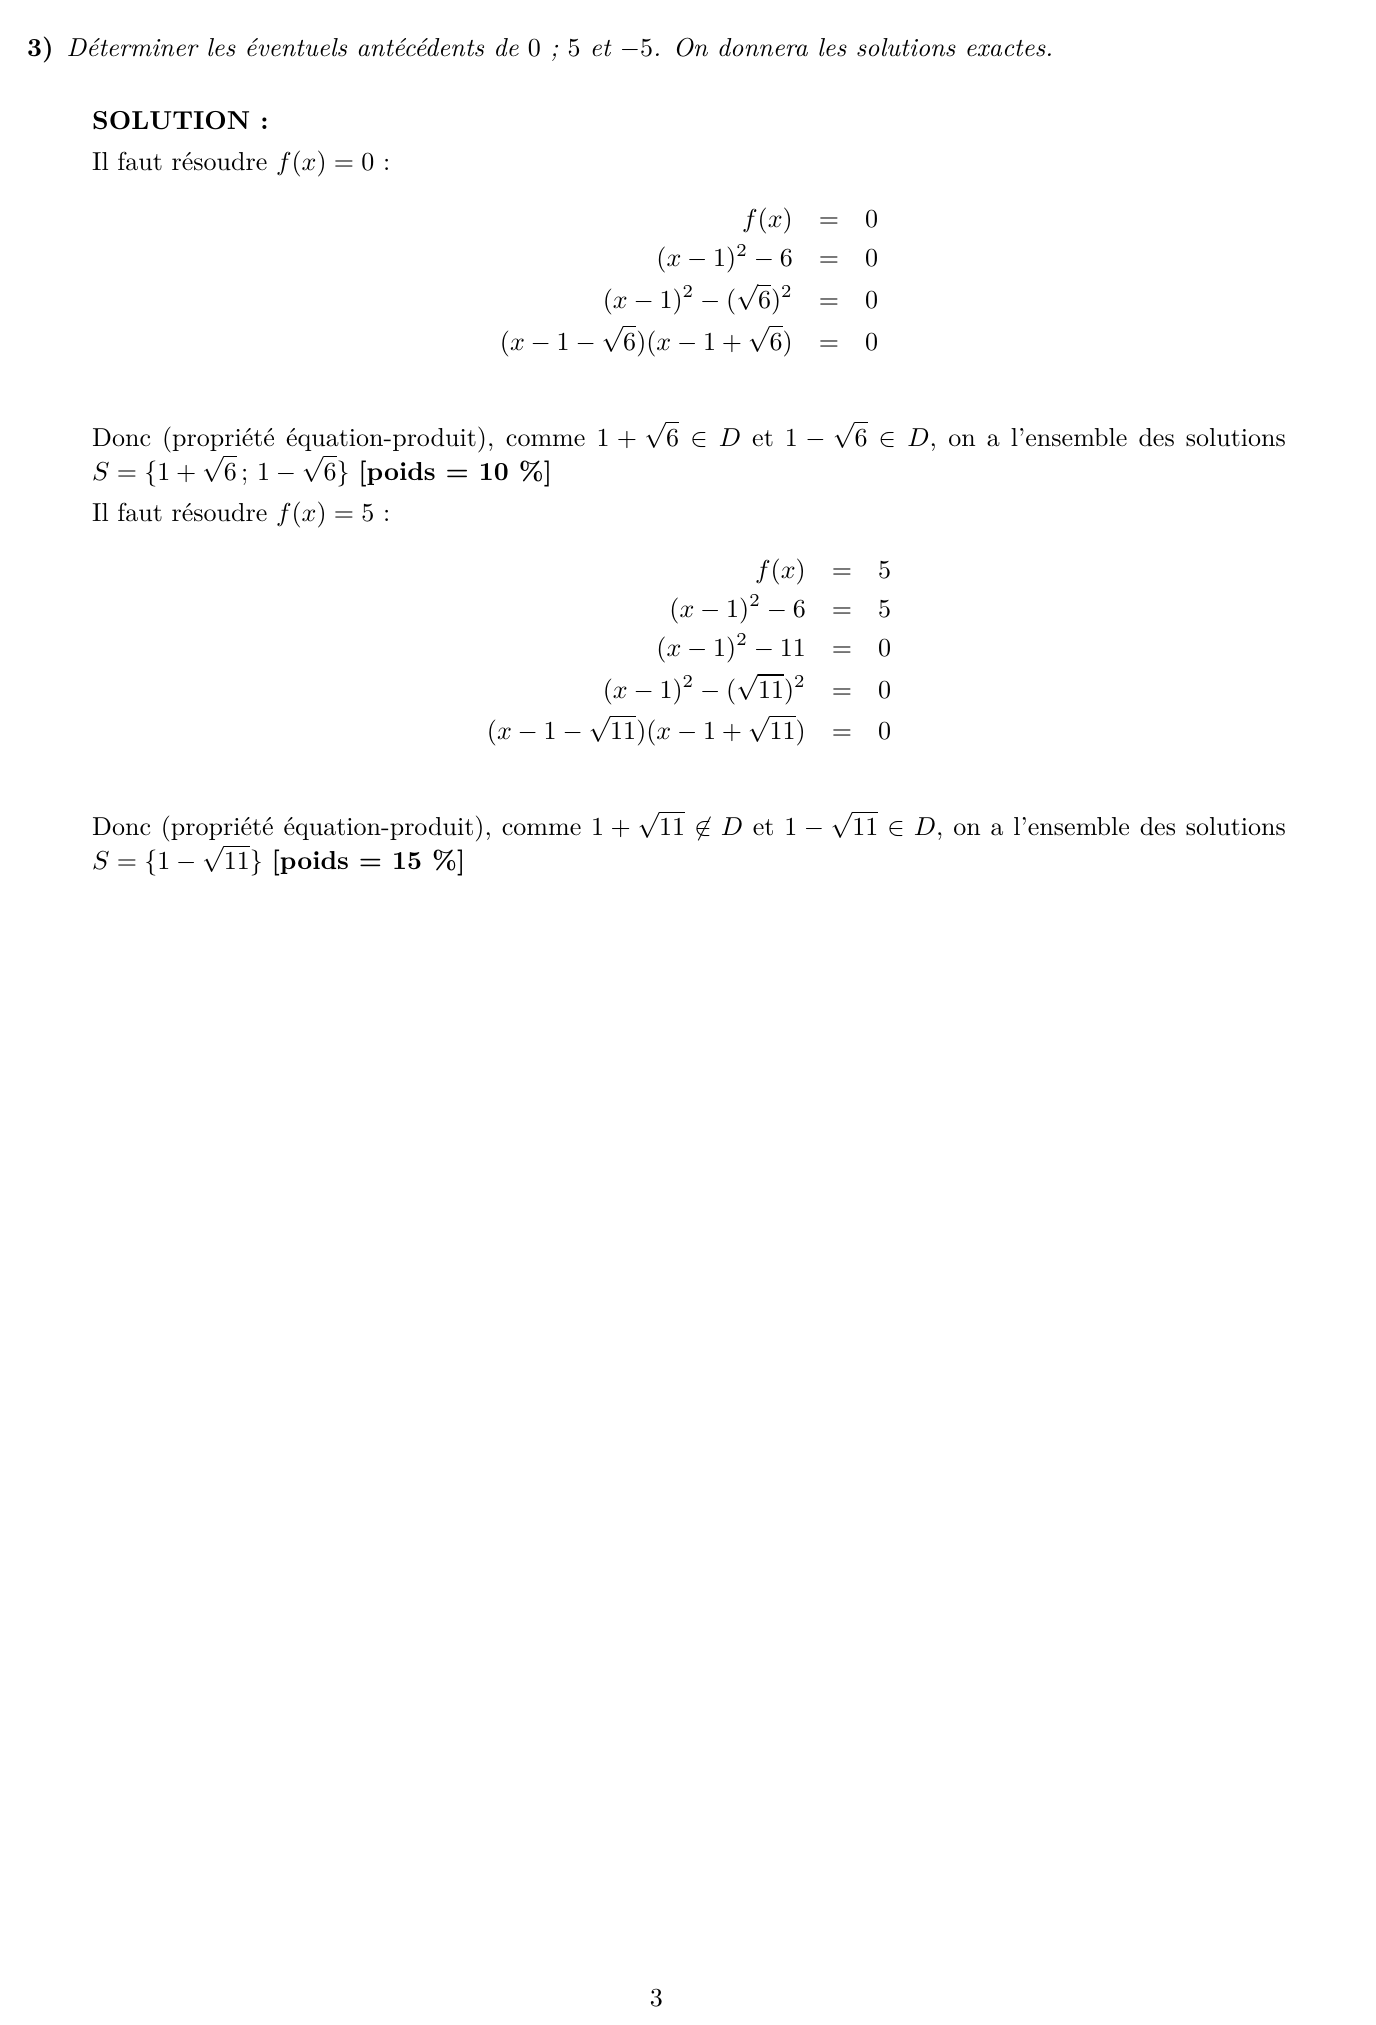
\includegraphics[width=5cm,height=7cm]{./images/creation_exercice_13.png}
\end{tabular}
\end{center}

\subsection{Etape 4 : Définir les variables qui changeront en fonction de l'énoncé}

Nous abordons ici la phase la plus cruciale de la création de variations de l'exercice. Pour cela il faut expliquer le rôle du bouton  \fbox{$\backslash$var$\{\}\{\}$} :

\begin{dsxl}
 Le rôle du bouton \fbox{$\backslash$var$\{\}\{\}$} \index[dsxlindex]{bouton  \fbox{$\backslash$var$\{\}\{\}$}} est le suivant : \\
Il identifie les valeurs numériques, les expressions, les équations qui sont variables dans l'énoncé. Le premier argument est le nom de la variable, 
  qui peut être une chaîne de caractères sans caractères spéciaux, comme $\%$, etc... \\
  Le second argument contient la part de texte qui sera modifiée. \\
  Par exemple $\backslash$var$\{delta\}\{5\}$ signifie que, à cet endroit du texte, le nombre $5$ correspond à la valeur de la variable $delta$ et, si plus tard $delta$ prend la valeur $6$,
  la valeur $5$ dans le texte sera remplacé par $6$. 

\end{dsxl}

Dans notre exemple d'exercice, le domaine de définition de $f$ est donné par $[-3 ; 4]$. Les valeurs de $-3$ et $4$ vont être variables et être nommées, respectivement, $xA$ et $yA$. 
Les deux extrémités de la courbe représentant $f$ sont les points $A(xA,yA)$ et $B(xB,yB)$. 
A l'évidence le code
\begin{verbatim}
 %C>
L'ensemble de définition est $D = [-3\,;\,4]$. \poids{5} %en pourcentage
%C<
\end{verbatim}
sera donc modifié en :
\begin{verbatim}
 %C>
L'ensemble de définition est $D = [\var{xA}{-3}\,;\,\var{xB}{4}]$. \poids{5} %en pourcentage
%C<
\end{verbatim}

Cliquons sur le bouton  \fbox{WRAP UP!} et compilons le fichier \\
{\bf DSXL\_3\_programme/dsxl\_tex\_exercice/latex\_wrapper\_in\_full/dsxl\_text\_latex\_wrapper\_out.tex}.

La partie concernée apparaît maintenant comme cela : 
\begin{figure}[h]
 \centering
 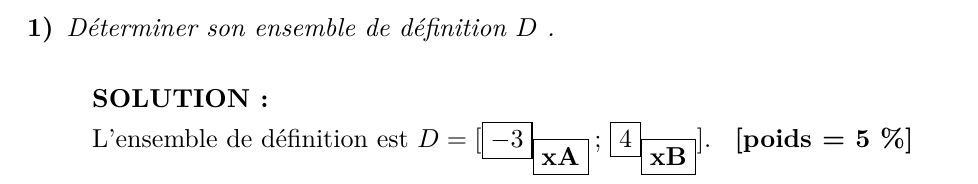
\includegraphics[width=12cm,height=2cm]{./images/creation_exercice_var_01.png}
 % creation_exercice_var_01.png: 978x184 px, 96dpi, 25.87x4.87 cm, bb=0 0 733 138
 \caption{Effet de $\backslash$var$\{\}\{\}$}
 \label{fig: var 01}
\end{figure}

\begin{remarque}
 Il est possible de voir la liste de toutes les les insertions en allant sur l'onglet \underline{python wrapper} et en regardant le menu déroulant à droite de {\bf Liste variables} :
 \begin{figure}[h]
 \centering
 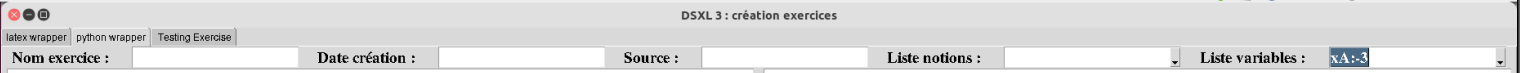
\includegraphics[width=18cm,height=1cm]{./images/creation_exercice_var_02.png}
 % creation_exercice_var_01.png: 978x184 px, 96dpi, 25.87x4.87 cm, bb=0 0 733 138
 \caption{Menu déroulant pour voir la liste des variables inserées}
 \label{fig: var 02}
\end{figure}
\end{remarque}

Les variables $xA$ et $yA$ doivent être substituées à d'autres endroits du texte. 
Voici la liste des passages concernés :
\begin{description}
 \item[a)] Le graphique :
 \begin{verbatim}
  \draw[line width=2.pt,smooth,samples=100,domain=-3.0:4.0] plot(\x,{(\x)^(2.0)-2*(\x)-5});
 \end{verbatim}
 et 
 \begin{verbatim}
 \draw [fill=black] (-3.,10.) circle (2.5pt);
\draw [fill=black] (4.0,3.) circle (2.5pt);
 \end{verbatim}
 \item[b)] La question 5) :
 \begin{verbatim}
  \item[5)]  
%E>
Résoudre graphiquement l'inéquation $f(x)\geq -3$.
%E<
%C>
Par lecture graphique on trouve $S = [-3\,;\,-0.7] \cup  [2.7\,;\,4]$ \poids{5} %en pourcentage
%C<
 \end{verbatim}
\item[c)] Le tableau de variations :
\begin{verbatim}
 \begin{center}
\begin{tabular}{|l|lllll|} \hline
$x$ & $-3$ &  & $1$ &  & $4$\\ \hline
 & $10$ &  &  &  & $3$\\ 
$f(x)$ &  & $\searrow$ &  & $\nearrow$ & \\
 &  &  & $-6$ &  & \\ \hline
\end{tabular}
\end{center}
\end{verbatim}

\end{description}




\begin{description}
 \item[Action pour le a) : ] 
 \index[dsxlindex]{$\backslash$var$\{\}\{\}$ dans un environnement graphique} 
\begin{bug} 
 Le remplacement de $-3$ par $\backslash$var$\{xA\}\{-3\}$ et  $4$ par $\backslash$var$\{xB\}\{4\}$ dans un environnements graphique est problématique, car la compilation ne se fera pas. 
 C'est pourquoi il faut procéder ici autrement :
 \begin{description}
  \item [1)] Dupliquer la ligne qui contiendra la commande (on aura deux fois la même ligne) et 
  \item[2)] insérer $\%$ au début de la ligne dupliquée. Puis insérer dans cette ligne les remplacements de $-3$ par $\backslash$var$\{xA\}\{-3\}$ et  $4$ par $\backslash$var$\{xB\}\{4\}$. 
  La compilation Latex se fera alors sans problème tout en permettant de faire apparaître les variables insérées (après clic sur \fbox{WRAP UP!}) .   
  \item[3)] A la fin de la création des variantes de l'exercice, il ne faudra pas oublier d'enlever $\%$ pour le remettre au début de la ligne non modifiée. 
  En effet, lors de l'utilisation de cet exercice dans un devoir la commande $\backslash$var$\{xB\}\{4\}$ disparaîtra pour 
  être remplacée pas la nouvelle valeur que prendra la variable $xA$ et la compilation Latex pourra se faire sans problème. 
 \end{description}
Le code du a) ci-dessus devient ainsi : 
 \begin{verbatim}
 %\draw[line width=2.pt,smooth,samples=100,domain=\var{xA}{-3}:\var{xB}{4.}] plot(\x,{(\x)^(2.0)-2*(\x)-5});
\draw[line width=2.pt,smooth,samples=100,domain=-3.0:4.0] plot(\x,{(\x)^(2.0)-2*(\x)-5});
 \end{verbatim}
 et 
 \begin{verbatim}
%\draw [fill=black] (\var{xA}{-3},10.) circle (2.5pt);
\draw [fill=black] (-3.,10.) circle (2.5pt);
%\draw [fill=black] (\var{xB}{4.},3.) circle (2.5pt);
\draw [fill=black] (4.0,3.) circle (2.5pt);
 \end{verbatim}
\end{bug}
 \item[Action pour le b) : ]  Dans cet exercice, le polynôme pourra avoir la forme $P(x) = ax^2+bx+c$ avec $a\in \{1;-1\}$. Cela implique que l'inéquation $P(x)\geq -3$ 
 ne sera pas forcement la réunion de deux intervalles. Il est donc plus approprié d'introduire la variable  $\backslash$var$\{ques5solS\}\{ [-3\,;\,-0.7] \backslash cup  [2.7\,;\,4]\}$ 
 pour obtenir la ligne :
 \begin{verbatim}
  %C>
Par lecture graphique on trouve $S =\var{ques5solS}{ [-3\,;\,-0.7] \cup  [2.7\,;\,4]}$ \poids{5} %en pourcentage
%C<
 \end{verbatim}
 Le nom de la variable doit être le plus pertinent possible. Cela facilitera beaucoup la suite du travail. 
 Après  clic sur \fbox{WRAP UP!} et compilation, on obtient :
  \begin{figure}[h]
 \centering
 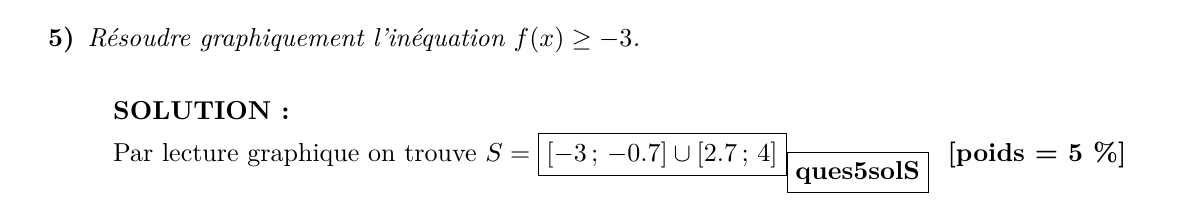
\includegraphics[width=15cm,height=2cm]{./images/creation_exercice_var_03b.png}
 % creation_exercice_var_01.png: 978x184 px, 96dpi, 25.87x4.87 cm, bb=0 0 733 138
 \caption{Résultat après  clic sur \fbox{WRAP UP!} et compilation}
 \label{fig: var 03b}
\end{figure}
 \item[Action pour le c) : ] La structure du tableau de variations ne changera pas, donc :
 \begin{verbatim}
  \begin{tabular}{|l|lllll|} \hline
$x$ & $\var{xA}{-3}$ &  & $1$ &  & $\var{xB}{4}$\\ \hline
 & $10$ &  &  &  & $3$\\ 
$f(x)$ &  & $\searrow$ &  & $\nearrow$ & \\
 &  &  & $-6$ &  & \\ \hline
\end{tabular}
 \end{verbatim}
  \begin{figure}[h]
 \centering
 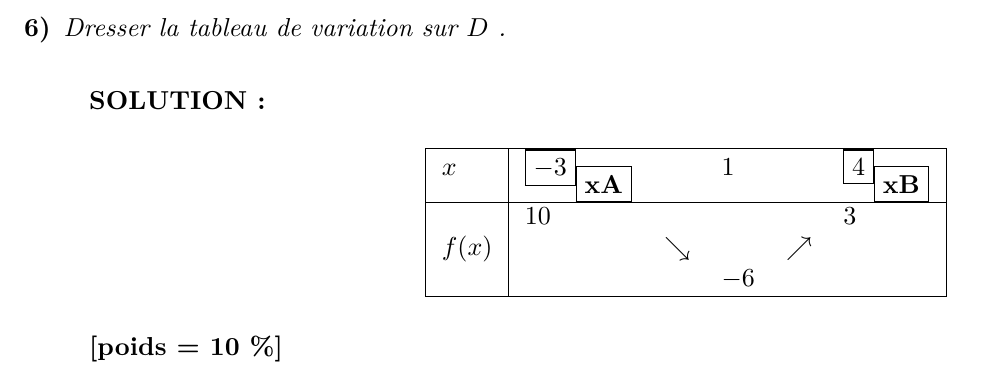
\includegraphics[width=10cm,height=3cm]{./images/creation_exercice_var_03c.png}
 % creation_exercice_var_01.png: 978x184 px, 96dpi, 25.87x4.87 cm, bb=0 0 733 138
 \caption{Résultat après  clic sur \fbox{WRAP UP!} et compilation}
 \label{fig: var 03c}
\end{figure}

\end{description}

\begin{remarque}
 Convention pour nommer les variables dans $\backslash$var$\{\}\{\}$ : \\
 Il est recommandé d'avoir des noms de variables pertinents (pA = partie A, pB = partie B, q1 = question 1, etc...)  : 
 \begin{center}
\begin{tabular}{llll}
Partie & Question & Nom de la variable & Valeur dans l'énoncé\\
A & 1 & sans objet & \\
A & 2 & ymaxpAq2,yminpAq2 & $10$ , $-6$\\
A & 3 a & ypAq3a & $-5 = f(0)$ (Lecture graphique de $f(0)$)\\
A & 3 b & xpAq3bsol1,xpAq3bsol2 & $−1.8$ , $3.7$\\
A & 3 b & ypAq3b2ant & $2$ (Choisir parmi les images qui ont 2 antécédents)\\
A & 4 a & ques4aSol & pour $x \approx 3.6$ et $x \approx −1.6$\\
A & 4 a & ypAq4a1ant & $1$ (Choisir parmi les images qui ont 1 antécédent)\\
A & 4 b & quespA4bSol & pour $x \approx -1.5$ et $x \approx 3.5$\\
A & 4 a & ypAq4b0ant & $0$ (Choisir parmi les images qui ont aucun antécédent)\\
A & 5 & ques5solS & \\
A & 5 & ypAq5 & $-3$\\
A & 6 & xA, x0, xB & $-3$, $1$, $4$\\
A & 6 & yA, y0, yB & $10$, $-6$, $3$\\
A & 6 & varGpAq6,  varDpAq6 & $\searrow$, $\nearrow$\\
 &  &  & \\
B&   & fdev & $ x^2-2x-5$\\
B&   & ftikz & $ \backslash x^2-2\backslash x-5$ fonction pour la représentation graphique. \\
B & 1 & f0pBq1, fm1pBq1, frac2pBq1 & Calcul des images de $0$, $-1$ et $\sqrt{2}$.\\
B & 2 & fcan & $(x-1)^2 -6 $\\
B & 2 & formecanpBq2et1 & Preuve de la forme canonique étape 1\\
B & 2 & formecanpBq2et2 & Preuve de la forme canonique étape 2\\
B & 3 & quespBq3sol2ant & \\
B & 3 & ypBq3deuxant & Image pour laquelle il y a deux antécédents\\
B & 3 & x1deuxant,x2deuxant & Les deux solutions\\
B & 3 & ensSdeuxant & Ensemble des solutions dans le domaine de définition. \\
B & 3 & quespBq3sol1ant & \\
B & 3 & ypBq3unant & Image pour laquelle il y a un antécédent \\
B & 3 & x1unant,x2unant & Les deux solutions\\
B & 3 & ensSunant & Ensemble des solutions dans le domaine de définition. 
 \end{tabular}
 \end{center}
 
\end{remarque}

La compilation de \\
{\bf\small DSXL\_3\_programme/dsxl\_tex\_exercice/latex\_wrapper\_in\_full/dsxl\_text\_latex\_wrapper\_out.tex}
en mode C donne :

 \begin{center}
 \begin{tabular}{ccc}
 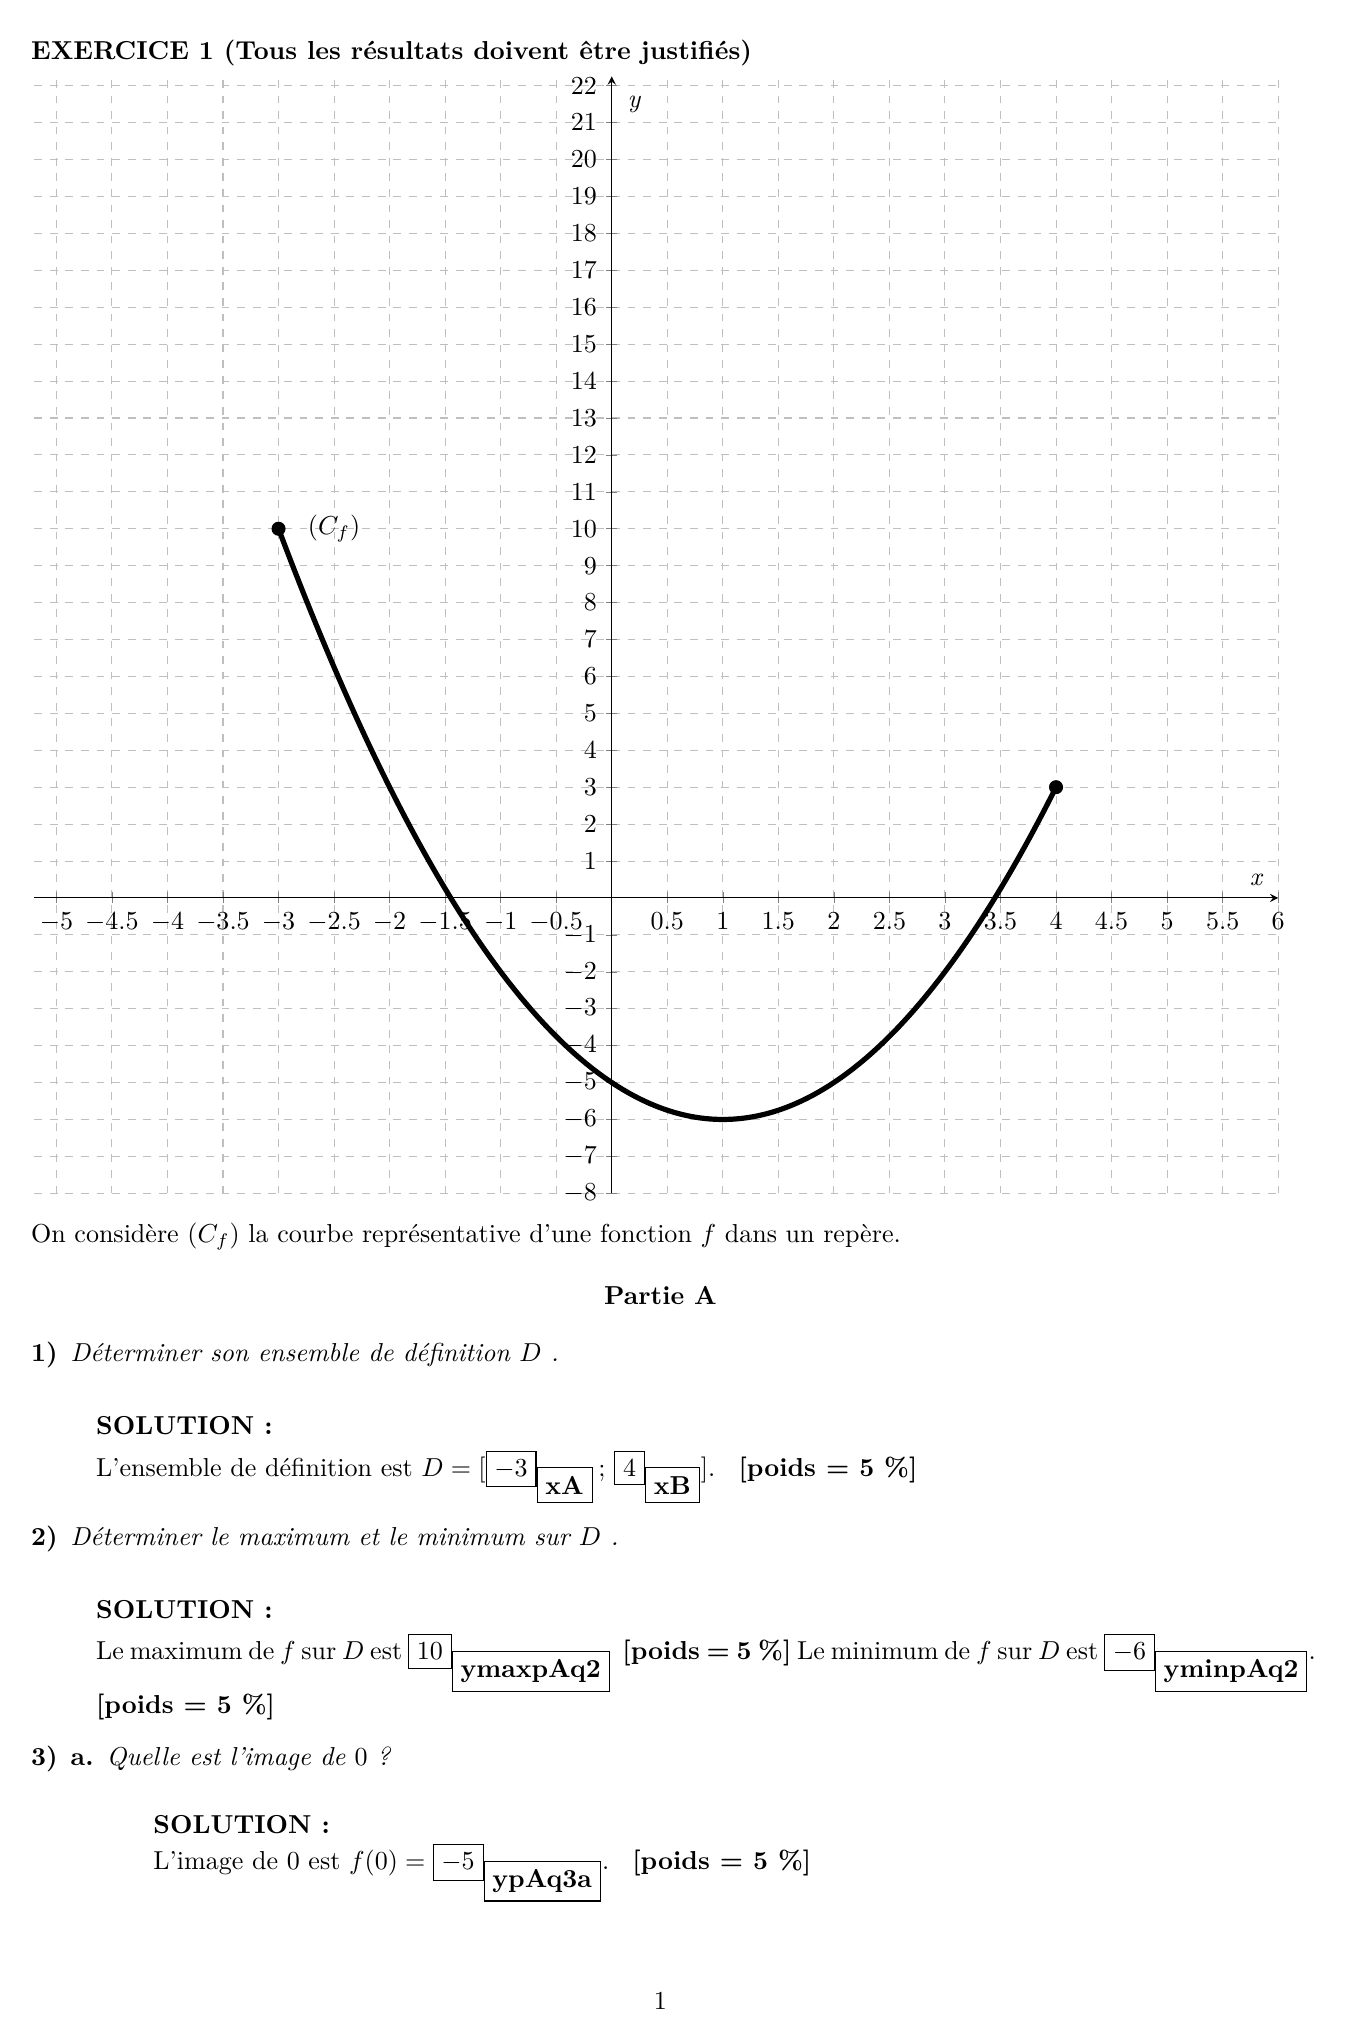
\includegraphics[width=5cm,height=7cm]{./images/creation_exercice_var_04a.png}
&
 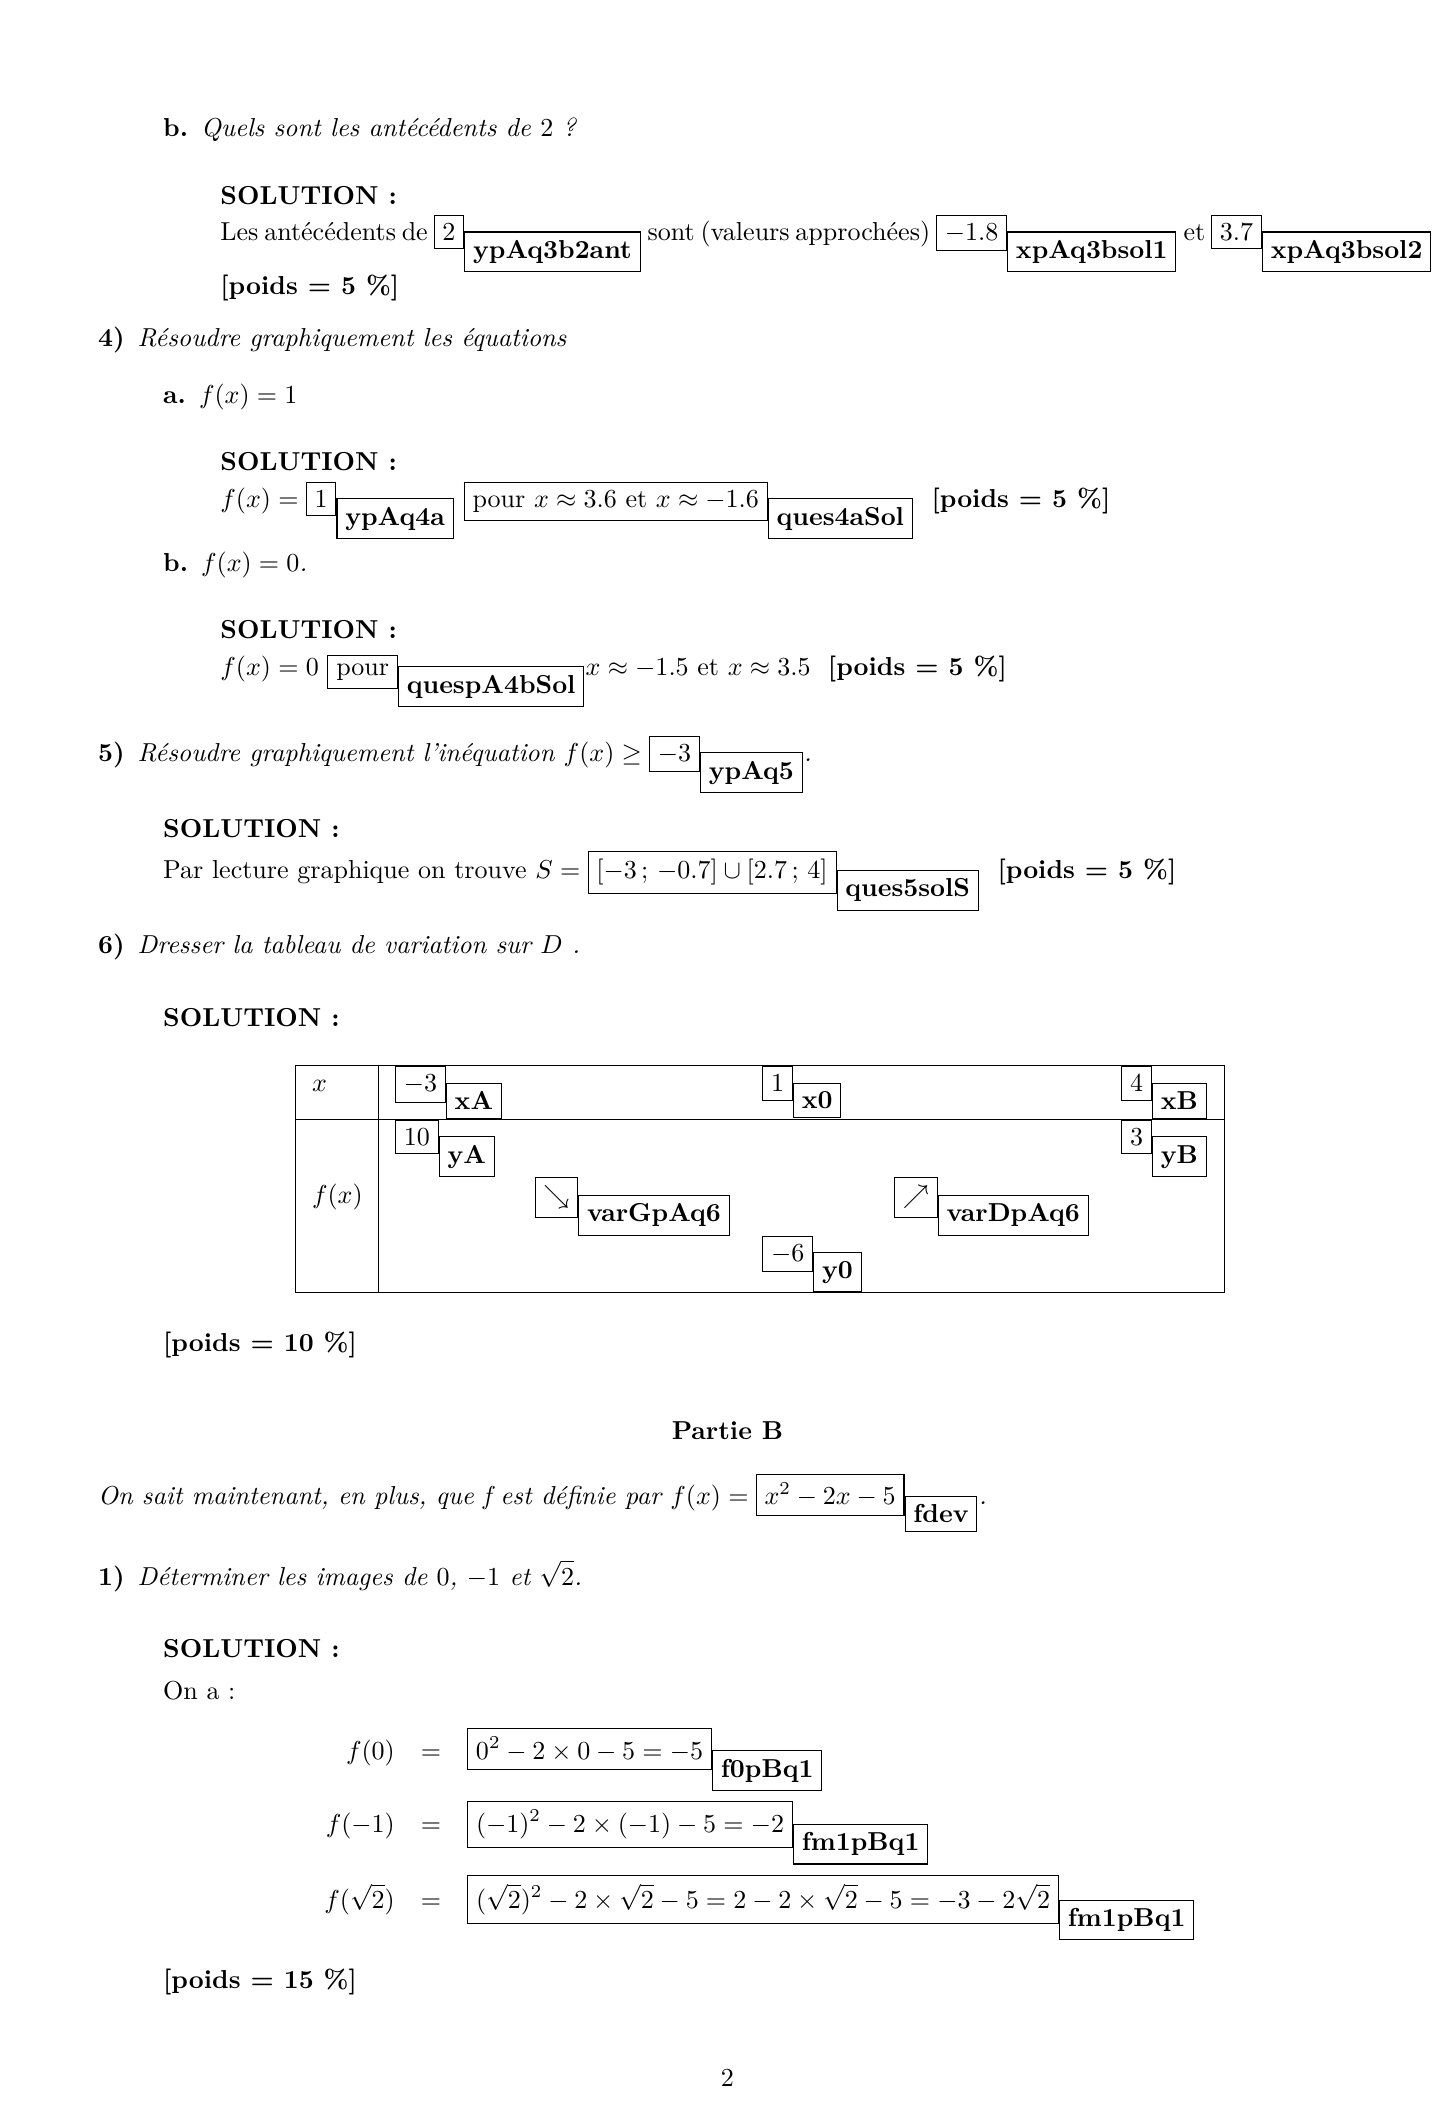
\includegraphics[width=5cm,height=7cm]{./images/creation_exercice_var_04b.png}
 &
 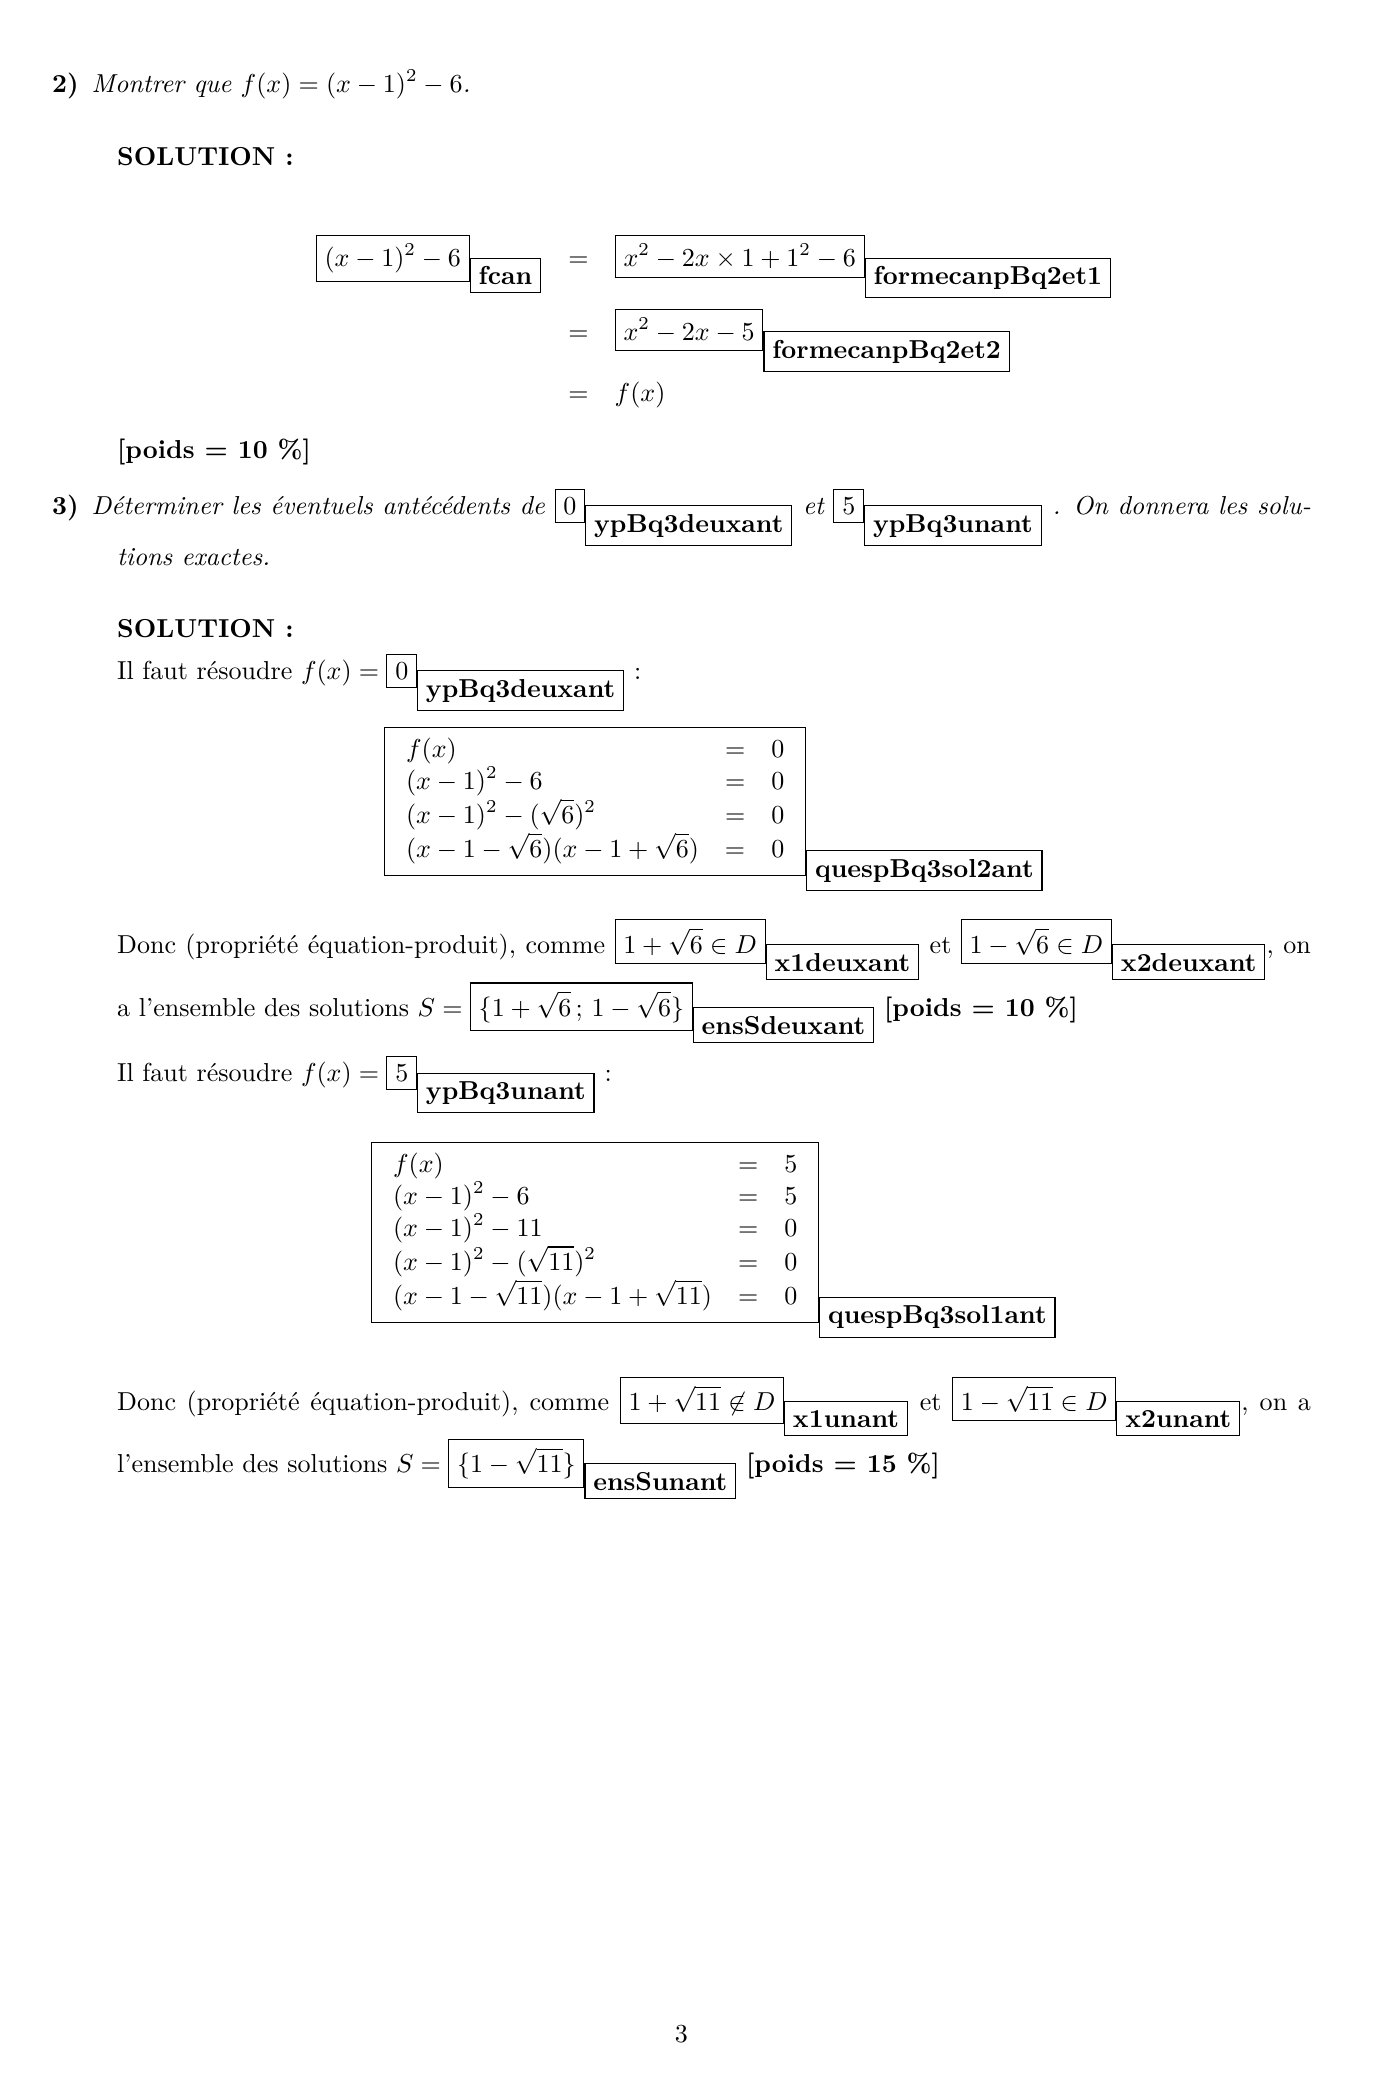
\includegraphics[width=5cm,height=7cm]{./images/creation_exercice_var_04c.png}
\end{tabular}
\end{center}

\begin{remarque} Quelques points importants : \\
\begin{enumerate}
 \item  Il ne faut pas oublier de modifier la fonction dans la partie graphique : 
 {\small
 \begin{verbatim}
%\draw[line width=2.pt,smooth,samples=100,domain=\var{xA}{-3}:\var{xB}{4.}] plot(\x,{\var{ftikz}{(\x)^(2.0)-2*(\x)-5}});
\draw[line width=2.pt,smooth,samples=100,domain=-3.0:4.0] plot(\x,{(\x)^(2.0)-2*(\x)-5});  
 \end{verbatim}
 }
\item Pour obtenir 
 \begin{center}
 \begin{tabular}{cc}
 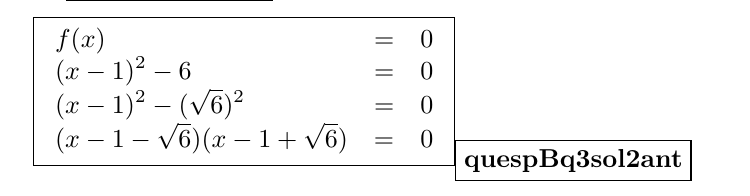
\includegraphics[width=8cm,height=3cm]{./images/creation_exercice_var_05a.png}
&
 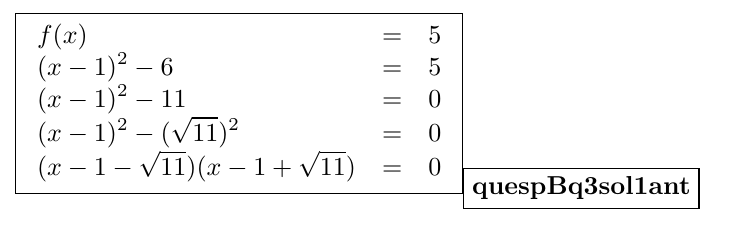
\includegraphics[width=8cm,height=3cm]{./images/creation_exercice_var_05b.png}
\end{tabular}
il est nécessaire de modifier quelque peu le code Latex, car $\backslash$var$\{\}\{\}$ nécessite d'être en mode mathématique :
\begin{verbatim*}
\begin{eqnarray*}
 f(x) &=& 0 \\
 (x-1)^2 -6  &=&0 \\
 (x-1)^2 -(\sqrt{6})^2  &=&0 \\
 (x-1-\sqrt{6})  (x-1+\sqrt{6}) &=&0 \\
\end{eqnarray*}

\end{verbatim*}
devient : 
\begin{verbatim*}
 $$
\var{quespBq3sol2ant}{
\begin{array}{lll}
 f(x) &=& 0 \\
 (x-1)^2 -6  &=&0 \\
 (x-1)^2 -(\sqrt{6})^2  &=&0 \\
 (x-1-\sqrt{6})  (x-1+\sqrt{6}) &=&0 \\
\end{array}
}
$$
\end{verbatim*}
Idem pour la seconde résolution. 
\end{center}
\end{enumerate}


\end{remarque}

\subsection{Etape 5 : Définir contraintes sur les variables et le fichier {\bf python\_contraintes.py}}
 Pour pouvoir continuer, il faut maintenant lister les contraintes que nos paramètres/variables vont devoir respecter : 

\begin{description}
\item[Partie A]
  \item[c1 : ] Valeurs minimales et maximales pour $x$ :  $xmin\leq x\leq xmax$ avec $xmin = -5$ et $xmax = 6$.
\item[c2 : ] Valeurs minimales et maximales pour $y$ :  $ymin\leq x\leq ymax$ avec $ymin = -8$ et $ymax = 22$.
\item[c3 A : ] Domaine de définition de $f$ : $xmin+margex\leq xA \leq -margex$ avec $margex = 2$. 
\item[c3 B : ] Domaine de définition de $f$ : $margex\leq xB \leq xmax-margex$ 
\item[Remarque : ] Avec c3 A et c3 B, on s'assure que $0$, $1$ et $\sqrt{2}$ sont dans le domaine de définition de $f$. 
\item[c4 A : ] Domaine images de $f$ : $ymin+margey\leq yA \leq ymax-margey$ avec $margey = 3$
\item[c4 B : ] Domaine images de $f$ : $ymin+margey\leq yB \leq ymax-margey$ avec $margey = 3$
\item[c5 : ] $yA \neq yB$ (Pour la partie B, 3) si on souhaite avoir la situation qu'une seule des solutions est dans le domaine de définition.)
\item[c6 : ] Minimum ($a=1$) ou maximum ($a=-1$) en $x0$ avec $xA +1\leq x0\leq xB-1$
\item[c7 : ] Pour $y0=f(x0)$ :  $ymin+margey\leq y0 \leq ymax-margey$
\item[c8 : ] Pour la question 3 b : Trouver les antécédents de $f(x) =  ypAq3b2ant $ avec \\
          $y0+1 \leq  ypAq3b2ant \leq \min\{yA,yB\}-1$ si $a=1$ et \\
          $  \max\{yA,yB\}+1\leq  ypAq3b2ant \leq y0-1$ si $a=-1$ (pour avoir toujours deux antécédents).
\item[c9 : ] Pour la question 4 on prendra un cas où il y a un antécédent et aucun antécédent : \\
          Antécédents de $f(x) =  ypAq4a1ant$ avec $\min\{yA,yB\}+1\leq y4a \leq \max\{yA,yB\}-1$ (Une solution)\\
          Antécédents de $f(x) = ypAq4a0ant$ avec $ymin+margey\leq y0 \leq \min\{yA,yB,y0\}-1$ ou 
           $ \max\{yA,yB,y0\}+1 \leq ypAq4a0ant \leq ymax-margey$ (aucune solution). 
\item[c inequation ] Pour la question 5 $f(x)\geq ypAq5$ avec deux antécédents  \\           
\item[Partie B]
\item[c10 a : ] Pour la question 3 : $f(x) = ypBq3deuxant$ avec :\\
    $y0+1 \leq ypBq3deuxant \leq \min\{yA,yB\}-1$ si $a=1$ et \\
          $  \max\{yA,yB\}+1\leq ypBq3deuxant \leq y0-1$ si $a=-1$ (pour avoir toujours deux antécédents).
\item[c10 b : ] Pour la question 3 : $f(x) = ypBq3unant$ avec $\min{yA,yB}+1\leq ypBq3unant\leq \max{yA,yB}-1$ (une solution)
 \end{description}
 
 Il reste à écrire quelques formules pour calculer $yA$, $yB$, $y0$. Le plus simple étant de prendre la forme canonique de $f$ :
 \begin{eqnarray*}
  f(x)&=& a (x-x_0)^2 - y_0 \mbox{ , alors : } \\
  y_A = f(x_A)&=& a(x_A-x_0)^2 - y_0 \mbox{ et }\\
  y_B =  f(x_B)&=& a(x_B-x_0)^2 - y_0
 \end{eqnarray*}

 
On peut maintenant écrire la procédure Python qui calculera toutes les combinaisons possibles :
{\small
\begin{verbatim}
# Nom du fichier \include{python_contraintes.py}
# Contraintes c1 et c2 :
xmin=-5
xmax=6
ymin=-8
ymax=22
margex = 2
margey = 3
# Variable pour compter le nombre d'énoncés différents : 
counter = 0
for xA in range(xmin+margex,-margex+1): #  Contrainte c3 A
    for xB in range(margex,xmax-margex+1): #  Contrainte c3 B 
        for x0 in range(xA+1,xB): #  Contrainte c6
            for a in [-1,1]: 
                if xA+xB!=2*x0: #  Contrainte c5
                    for y0 in range(ymin+margey,ymax-margey+1): #  Contrainte c7
                        yA = a*(xA-x0)**2+y0
                        yB = a*(xB-x0)**2+y0
                        if (yB>ymin+margey) and (yB<ymax-margey) and (yA>ymin+margey) and (yA<ymax-margey) :  
                            # On définit les listes pour les images ayant 0, 1 et 2 antécédents : 
                            list_y_0_sol = []
                            list_y_1_sol = []
                            list_y_2_sol = []
                            for y in range(ymin+margey,ymax-margey+1) : 
                                if y< min(yA,yB,y0) or y> max(yA,yB,y0) :
                                    list_y_0_sol.append(y)
                                if y>min(yA,yB) and y<max(yA,yB) :
                                    list_y_1_sol.append(y)
                                if (a==1) and (y>y0) and (y<min(yA,yB)) : 
                                    list_y_2_sol.append(y)
                                if (a==-1) and (y<y0) and (y>max(yA,yB)) : 
                                    list_y_2_sol.append(y) 
                                # La condition suivante permet juste de restreindre le nombre de possibilités en imposant un nombre minimal de solutions : 
                                if not(len(list_y_0_sol)<5 or len(list_y_1_sol)<5 or len(list_y_2_sol)<5) : 
                                    print('A(',xA,' , ',yA,' ) B( ',xB,' , ',yB,' ) , P ( ', x0,' , ',y0,' ) \
                                    avec a = ', a, ' f(x) = ',a,' [x - ( ',x0,' )]^2 - ( ',y0,' )' )
                                    print('list_y_0_sol =',list_y_0_sol)
                                    print('list_y_1_sol =',list_y_1_sol)
                                    print('list_y_2_sol =',list_y_2_sol)
                                    counter = counter+1
                                    
print('counter = ',counter)
\end{verbatim}
}

Le programme ci-dessus permet donc de générer au moins $56$ possibilités de tuples de valeurs pour $a$, $xA$, $xB$, $x0$, $yA$, $yB$, $y0$ et au moins : 
\begin{description}
 \item[len(list\_y\_0\_sol) $\geq 5$] possibilités pour $y4b$ (aucune solution)
  \item[len(list\_y\_1\_sol )$\geq 5$] possibilités pour , $y4a$, $ypB3b$ (une solution)
 \item[len(list\_y\_2\_sol) $\geq 5$] possibilités pour $y3b$, $ypB3a$, $y5$ (deux solutions)
\end{description}

Cela fait au moins $56\times 5^3 = 7000$ énoncés différents!

Les variables peuvent maintenant être separées en deux groupes : 

\begin{description}
 \item[Les valeurs libres :] Celles qui sont générées par le programme ci-dessus ( $python\_contraintes.py$ ) 
 \begin{verbatim}
  r'xA:-3' , 
  r'xB:4.' , 
  r'x0:1' ,
  r'y0:-6' ,  
  'yminpAq2:-6' ,   
  'ypAq3b2ant:2'  , # Elément de list_y_2_sol
  r'ypAq4a1ant:1' , # Elément de list_y_1_sol
  r'ypAq5:-3' ,     # Elément de list_y_2_sol
  r'ypAq4a0ant:0' , # Elément de list_y_0_sol
 \end{verbatim}

 \item[Les valeurs calculées à partir des valeurs libres : ] 
 \begin{verbatim}
  r'ypAq3a:-5' , 
  r'ftikz:(\x)^(2.0)-2*(\x)-5' , 
  r'ymaxpAq2:10' ,  
  'xpAq3bsol1:-1.8' , 'xpAq3bsol2:3.7' ,
  r'ques4aSol:\mbox{pour }x\approx 3.6\mbox{ et }x\approx -1.6' ,  
  r'quespA4bSol:\mbox{pour}x\approx -1.5\mbox{ et }x\approx 3.5' , 
  r'ques5solS: [-3\,;\,-0.7] \cup  [2.7\,;\,4]' , , 
  r'varGpAq6:\searrow' , 'varDpAq6:\nearrow' ,  
  r'fdev: x^2-2 x -5' , 
  r'f0pBq1: 0^2 - 2 \times 0 -5 = -5 ' , 
  r'fm1pBq1:(-1)^2 - 2 \times (-1) -5 = -2' , 
  r'fcan:(x-1)^2 -6' , 
  r'formecanpBq2et1:x^2 - 2 x\times 1 + 1^2 - 6' , 
  r'formecanpBq2et2:x^2 - 2 x -5 ' , 
  r'ypBq3deuxant:0' , 'ypBq3unant:5' , 
  r'quespBq3sol2ant:\begin{array}{lll} f(x) &=& 0 \\ (x-1)^2 -6  &=&0 \\ (x-1)^2-(\sqrt{6})^2  &=&0 \\ (x-1-\sqrt{6})  (x-1+\sqrt{6}) &=&0 \\\end{array}' , 
  r'x1deuxant:1+\sqrt{6}\in D' , 'x2deuxant:1-\sqrt{6}\in D' , 
  r'ensSdeuxant:\{1+\sqrt{6} \,;\,1-\sqrt{6} \}' , 
  r'quespBq3sol1ant:\begin{array}{lll} f(x) &=&5 \\ (x-1)^2 -6  &=&5 \\  (x-1)^2 -11  &=&0 \\ (x-1)^2 -(\sqrt{11})^2  &=&0 \\ (x-1-\sqrt{11})  (x-1+\sqrt{11}) &=&0\end{array}' ,
  r'x1unant:1+\sqrt{11}\not\in D' , 'x2unant:1-\sqrt{11}\in D' , 
  r'ensSunant: \{1-\sqrt{11} \}'    
 \end{verbatim}

\end{description}


\section{L'onglet \underline{python wrapper}}
\subsection{Etape 6 : Définir la fonction def $fonction\_param\_exercice()$ : }

Pour cela il faut aller sur l'onglet \underline{python wrapper} et cliquer sur le bouton \fbox{Nouvelle fonction python}. 
Ensuite deux fois répondre oui au messages qui se présentent. 

Le programme génère alors un caneva (prototype) de programme qu'il faudra copier et coller dans un fichier python que l'on pourra appeler
{\bf $fonction\_param\_exercice\_raw.py$} par exemple (raw signifiant brute).

Pour des exercices simples, ce fichier peut déjà être compiler sans erreurs. Ici, ce n'est pas le cas, car l'exemple a été choisi pour contenir la plus grande 
majorité des situations que l'on peut rencontrer lors de la création d'un exercice. 

La première chose est de mettre en forme le dictionnaire {\bf  $dico\_exercice$} :
\begin{verbatim}
 def fonction_param_exercice() : 

    dico_exercice = {
        'nom_exercice': 'exercice_004' ,
        'date_creation': '12/03/2024' ,
        'source': 'Marcus' ,
        'liste_notions' :  [ '2nd' , 'développement' , 'fonction polynôme' , 'lecture graphique' , 'maximum' , 'tableau de variations' ] , 
        'liste_variables' :  [ 'xA:-3' , 
                              'xB:4.' , 
                              'ftikz:(\x)^(2.0)-2*(\x)-5' , 
                              'ymaxpAq2:10' , 'yminpAq2:-6' , 
                              'ypAq3a:-5' , 'ypAq3b2ant:2' , 'xpAq3bsol1:-1.8' , 'xpAq3bsol2:3.7' ,
                              'ypAq4a1ant:1' , 
                              'ques4aSol:\mbox{pour }x\approx 3.6\mbox{ et }x\approx -1.6' , 
                              'ypAq4a0ant:0' , 
                              'quespA4bSol:\mbox{pour}x\approx -1.5\mbox{ et }x\approx 3.5' , 
                              'ypAq5:-3' , 
                              'ques5solS: [-3\,;\,-0.7] \cup  [2.7\,;\,4]' , 
                              'x0:1' , 'yA:10' , 'yB:3' , 
                              'varGpAq6:\searrow' , 'varDpAq6:\nearrow' , 
                              'y0:-6' , 
                              'fdev: x^2-2 x -5' , 
                              'f0pBq1: 0^2 - 2 \times 0 -5 = -5 ' , 
                              'fm1pBq1:(-1)^2 - 2 \times (-1) -5 = -2' , 
                              'fcan:(x-1)^2 -6' , 
                              'formecanpBq2et1:x^2 - 2 x\times 1 + 1^2 - 6' , 
                              'formecanpBq2et2:x^2 - 2 x -5 ' , 
                              'ypBq3deuxant:0' , 'ypBq3unant:5' , 
                              'quespBq3sol2ant:\begin{array}{lll} f(x) &=& 0 \\ (x-1)^2 -6  &=&0 \\ (x-1)^2-(\sqrt{6})^2  &=&0 \\ (x-1-\sqrt{6})  (x-1+\sqrt{6}) &=&0 \\\end{array}' , 
                              'x1deuxant:1+\sqrt{6}\in D' , 'x2deuxant:1-\sqrt{6}\in D' , 
                              'ensSdeuxant:\{1+\sqrt{6} \,;\,1-\sqrt{6} \}' , 
                              'quespBq3sol1ant:\begin{array}{lll} f(x) &=&5 \\ (x-1)^2 -6  &=&5 \\  (x-1)^2 -11  &=&0 \\ (x-1)^2 -(\sqrt{11})^2  &=&0 \\ (x-1-\sqrt{11})  (x-1+\sqrt{11}) &=&0\end{array}' ,
                              'x1unant:1+\sqrt{11}\not\in D' , 'x2unant:1-\sqrt{11}\in D' , 
                              'ensSunant: \{1-\sqrt{11} \}' ]
        }
\end{verbatim}

Si on essaye de compiler, on obtient le message d'erreur suivant : 

\begin{verbatim} 
Input In [1]
    'ftikz:(\x)^(2.0)-2*(\x)-5' ,
                                ^
SyntaxError: (unicode error) 'unicodeescape' codec can't decode bytes in position 7-8: truncated \xXX escape 
\end{verbatim}

Ce problème est du à l'interpretation de $\backslash$ x. Pour résoudre ce problème, il suffit de modifier la ligne
\begin{verbatim}
 'ftikz:(\x)^(2.0)-2*(\x)-5' , 
\end{verbatim}
en 
\begin{verbatim}
 r'ftikz:(\x)^(2.0)-2*(\x)-5' , 
\end{verbatim}

Pour plus d'explications sur \index{dsxlindex}{unicode error}, voir : \url{https://www.digitalocean.com/community/tutorials/python-raw-string}

Il faut procéder ainsi pour toutes les chaines de caractère (indispensable pour celles ne sont pas numériques et à mettre avant ces chaînes de caractères 
(surtout si elles contiennent les séquences $\backslash$a (qui sera visualisé par le logo d'un téléphone), 
$\backslash$t (qui sera interprété par un tabular), etc...) un {\bf r}. 


La prochaine erreur de compilation python concerne la liste 
\begin{verbatim}
 liste_liste_parametres
\end{verbatim}

Pour résoudre ce problème, il suffit d'effacer l'item présent dans cette liste et de le remplacer par la valeur de 
\begin{verbatim}
 dico_exercice['liste_variables'] 
\end{verbatim}
On a : 

\begin{verbatim}
    liste_liste_parametres = [  [ r'xA:-3' , 
                              r'xB:4.' , 
                              r'ftikz:(\x)^(2.0)-2*(\x)-5' , 
                              r'ymaxpAq2:10' , 'yminpAq2:-6' , 
                              r'ypAq3a:-5' , 'ypAq3b2ant:2' , 'xpAq3bsol1:-1.8' , 'xpAq3bsol2:3.7' ,
                              r'ypAq4a1ant:1' , 
                              r'ques4aSol:\mbox{pour }x\approx 3.6\mbox{ et }x\approx -1.6' , 
                              r'ypAq4a0ant:0' , 
                              r'quespA4bSol:\mbox{pour}x\approx -1.5\mbox{ et }x\approx 3.5' , 
                              r'ypAq5:-3' , 
                              r'ques5solS: [-3\,;\,-0.7] \cup  [2.7\,;\,4]' , 
                              r'x0:1' , 'yA:10' , 'yB:3' , 
                              r'varGpAq6:\searrow' , 'varDpAq6:\nearrow' , 
                              r'y0:-6' , 
                              r'fdev: x^2-2 x -5' , 
                              r'f0pBq1: 0^2 - 2 \times 0 -5 = -5 ' , 
                              r'fm1pBq1:(-1)^2 - 2 \times (-1) -5 = -2' , 
                              r'fcan:(x-1)^2 -6' , 
                              r'formecanpBq2et1:x^2 - 2 x\times 1 + 1^2 - 6' , 
                              r'formecanpBq2et2:x^2 - 2 x -5 ' , 
                              r'ypBq3deuxant:0' , 'ypBq3unant:5' , 
                              r'quespBq3sol2ant:\begin{array}{lll} f(x) &=& 0 \\ (x-1)^2 -6  &=&0 \\ (x-1)^2-(\sqrt{6})^2  &=&0 \\ (x-1-\sqrt{6})  (x-1+\sqrt{6}) &=&0 \\\end{array}' , 
                              r'x1deuxant:1+\sqrt{6}\in D' , 'x2deuxant:1-\sqrt{6}\in D' , 
                              r'ensSdeuxant:\{1+\sqrt{6} \,;\,1-\sqrt{6} \}' , 
                              r'quespBq3sol1ant:\begin{array}{lll} f(x) &=&5 \\ (x-1)^2 -6  &=&5 \\  (x-1)^2 -11  &=&0 \\ (x-1)^2 -(\sqrt{11})^2  &=&0 \\ (x-1-\sqrt{11})  (x-1+\sqrt{11}) &=&0\end{array}' ,
                              r'x1unant:1+\sqrt{11}\not\in D' , 'x2unant:1-\sqrt{11}\in D' , 
                              r'ensSunant: \{1-\sqrt{11} \}' ]] 
\end{verbatim} 


\begin{dsxl} La liste
 \begin{verbatim}
 liste_liste_parametres
\end{verbatim}
va jouer un rôle crucial, car elle contiendra la liste de toutes les listes de valeurs possibles pour nos paramètres : \\
Chaque élément de cette liste est elle même une liste qui contient pour chaque paramètre/variable définie une valeur qui sera remplacée dans le texte de l'exercice. 
\end{dsxl}

La compilation s'arrête à l'erreur suivante : 

\begin{verbatim}
 Input In [4]
    ftikz = (\x)^(2.0)-2*(\x)-5
              ^
SyntaxError: unexpected character after line continuation character
\end{verbatim}

On procède au mêmes corrections que ci-dessus et on obtient : 

Le Résultat est :
\begin{verbatim}
    # Votre code ici :

    xA = -3 
    str_xA = str(xA) 
    xB = 4. 
    str_xB = str(xB) 
    ftikz = r'(\x)^(2.0)-2*(\x)-5' 
    str_ftikz = str(ftikz) 
    ymaxpAq2 = 10 
    str_ymaxpAq2 = str(ymaxpAq2) 
    yminpAq2 = -6 
    str_yminpAq2 = str(yminpAq2) 
    ypAq3a = -5 
    str_ypAq3a = str(ypAq3a) 
    ypAq3b2ant = 2 
    str_ypAq3b2ant = str(ypAq3b2ant) 
    xpAq3bsol1 = -1.8 
    str_xpAq3bsol1 = str(xpAq3bsol1) 
    xpAq3bsol2 = 3.7 
    str_xpAq3bsol2 = str(xpAq3bsol2) 
    ypAq4a1ant = 1 
    str_ypAq4a1ant = str(ypAq4a1ant) 
    ques4aSol = r'\mbox{pour }x\approx 3.6\mbox{ et }x\approx -1.6' 
    str_ques4aSol = str(ques4aSol) 
    ypAq4a0ant = 0 
    str_ypAq4a0ant = str(ypAq4a0ant) 
    quespA4bSol = r'\mbox{pour}x\approx -1.5\mbox{ et }x\approx 3.5' 
    str_quespA4bSol = str(quespA4bSol) 
    ypAq5 = -3 
    str_ypAq5 = str(ypAq5) 
    ques5solS =  r'[-3\,;\,-0.7] \cup  [2.7\,;\,4]' 
    str_ques5solS = str(ques5solS) 
    x0 = 1 
    str_x0 = str(x0) 
    yA = 10 
    str_yA = str(yA) 
    yB = 3 
    str_yB = str(yB) 
    varGpAq6 = r'\searrow'
    str_varGpAq6 = str(varGpAq6) 
    varDpAq6 = r'\nearrow' 
    str_varDpAq6 = str(varDpAq6) 
    y0 = -6 
    str_y0 = str(y0) 
    fdev =  r'x^2-2 x -5' 
    str_fdev = str(fdev) 
    f0pBq1 =  r'0^2 - 2 \times 0 -5 = -5'  
    str_f0pBq1 = str(f0pBq1) 
    fm1pBq1 = r'(-1)^2 - 2 \times (-1) -5 = -2' 
    str_fm1pBq1 = str(fm1pBq1) 
    fcan = '(x-1)^2 -6' 
    str_fcan = str(fcan) 
    formecanpBq2et1 = r'x^2 - 2 x\times 1 + 1^2 - 6' 
    str_formecanpBq2et1 = str(formecanpBq2et1) 
    formecanpBq2et2 = r'x^2 - 2 x -5'  
    str_formecanpBq2et2 = str(formecanpBq2et2) 
    ypBq3deuxant = 0 
    str_ypBq3deuxant = str(ypBq3deuxant) 
    ypBq3unant = 5 
    str_ypBq3unant = str(ypBq3unant) 
    quespBq3sol2ant = r'\begin{array}{lll}  f(x) &=& 0 \\  (x-1)^2 -6  &=&0 \\  (x-1)^2 -(\sqrt{6})^2  &=&0 \\  (x-1-\sqrt{6})  (x-1+\sqrt{6}) &=&0 \\ \end{array}'
 
    str_quespBq3sol2ant = str(quespBq3sol2ant) 
    x1deuxant = r'1+\sqrt{6}\in D' 
    str_x1deuxant = str(x1deuxant) 
    x2deuxant = r'1-\sqrt{6}\in D' 
    str_x2deuxant = str(x2deuxant) 
    ensSdeuxant = r'\{1+\sqrt{6} \,;\,1-\sqrt{6} \}' 
    str_ensSdeuxant = str(ensSdeuxant) 
    quespBq3sol1ant = r'\begin{array}{lll} f(x) &=&5 \\  (x-1)^2 -6  &=&5 \\   (x-1)^2 -11  &=&0 \\  (x-1)^2 -(\sqrt{11})^2  &=&0 \\  (x-1-\sqrt{11})  (x-1+\sqrt{11}) &=&0 \end{array}'
 
    str_quespBq3sol1ant = str(quespBq3sol1ant) 
    x1unant = r'1+\sqrt{11}\not\in D' 
    str_x1unant = str(x1unant) 
    x2unant = r'1-\sqrt{11}\in D' 
    str_x2unant = str(x2unant) 
    ensSunant =  r'\{1-\sqrt{11} \}' 
    str_ensSunant = str(ensSunant) 
\end{verbatim}

La compilation python devrait maintenant se faire sans problème.

 On obtient :
 {\tiny
\begin{verbatim}
valeurs par defaut --> xA:-3 | xA:-3  <---votre valeur : 
valeurs par defaut --> xB:4. | xB:4.0  <---votre valeur : 
valeurs par defaut --> ftikz:(\x)^(2.0)-2*(\x)-5 | ftikz:(\x)^(2.0)-2*(\x)-5  <---votre valeur : 
valeurs par defaut --> ymaxpAq2:10 | ymaxpAq2:10  <---votre valeur : 
valeurs par defaut --> yminpAq2:-6 | yminpAq2:-6  <---votre valeur : 
valeurs par defaut --> ypAq3a:-5 | ypAq3a:-5  <---votre valeur : 
valeurs par defaut --> ypAq3b2ant:2 | ypAq3b2ant:2  <---votre valeur : 
valeurs par defaut --> xpAq3bsol1:-1.8 | xpAq3bsol1:-1.8  <---votre valeur : 
valeurs par defaut --> xpAq3bsol2:3.7 | xpAq3bsol2:3.7  <---votre valeur : 
valeurs par defaut --> ypAq4a1ant:1 | ypAq4a1ant:1  <---votre valeur : 
valeurs par defaut --> ques4aSol:\mbox{pour }x\approx 3.6\mbox{ et }x\approx -1.6 | ques4aSol:\mbox{pour }x\approx 3.6\mbox{ et }x\approx -1.6  <---votre valeur : 
valeurs par defaut --> ypAq4a0ant:0 | ypAq4a0ant:0  <---votre valeur : 
valeurs par defaut --> quespA4bSol:\mbox{pour}x\approx -1.5\mbox{ et }x\approx 3.5 | quespA4bSol:\mbox{pour}x\approx -1.5\mbox{ et }x\approx 3.5  <---votre valeur : 
valeurs par defaut --> ypAq5:-3 | ypAq5:-3  <---votre valeur : 
valeurs par defaut --> ques5solS: [-3\,;\,-0.7] \cup  [2.7\,;\,4] | ques5solS:[-3\,;\,-0.7] \cup  [2.7\,;\,4]  <---votre valeur : 
valeurs par defaut --> x0:1 | x0:1  <---votre valeur : 
valeurs par defaut --> yA:10 | yA:10  <---votre valeur : 
valeurs par defaut --> yB:3 | yB:3  <---votre valeur : 
valeurs par defaut --> varGpAq6:\searrow | varGpAq6:\searrow  <---votre valeur : 
valeurs par defaut --> varDpAq6:
earrow | varDpAq6:\nearrow  <---votre valeur : 
valeurs par defaut --> y0:-6 | y0:-6  <---votre valeur : 
valeurs par defaut --> fdev: x^2-2 x -5 | fdev:x^2-2 x -5  <---votre valeur : 
valeurs par defaut --> f0pBq1: 0^2 - 2 \times 0 -5 = -5  | f0pBq1:0^2 - 2 \times 0 -5 = -5  <---votre valeur : 
valeurs par defaut --> fm1pBq1:(-1)^2 - 2 \times (-1) -5 = -2 | fm1pBq1:(-1)^2 - 2 \times (-1) -5 = -2  <---votre valeur : 
valeurs par defaut --> fcan:(x-1)^2 -6 | fcan:(x-1)^2 -6  <---votre valeur : 
valeurs par defaut --> formecanpBq2et1:x^2 - 2 x\times 1 + 1^2 - 6 | formecanpBq2et1:x^2 - 2 x\times 1 + 1^2 - 6  <---votre valeur : 
valeurs par defaut --> formecanpBq2et2:x^2 - 2 x -5  | formecanpBq2et2:x^2 - 2 x -5  <---votre valeur : 
valeurs par defaut --> ypBq3deuxant:0 | ypBq3deuxant:0  <---votre valeur : 
valeurs par defaut --> ypBq3unant:5 | ypBq3unant:5  <---votre valeur : 
valeurs par defaut --> quespBq3sol2ant:\begin{array}{lll} f(x) &=& 0 \\ (x-1)^2 -6  &=&0 \\ (x-1)^2-(\sqrt{6})^2  &=&0 \\ (x-1-\sqrt{6})  (x-1+\sqrt{6}) &=&0 \\\end{array} | quespBq3sol2ant:\begin{array}{lll}  f(x) &=& 0 \\  (x-1)^2 -6  &=&0 \\  (x-1)^2 -(\sqrt{6})^2  &=&0 \\  (x-1-\sqrt{6})  (x-1+\sqrt{6}) &=&0 \\ \end{array}  <---votre valeur : 
valeurs par defaut --> x1deuxant:1+\sqrt{6}\in D | x1deuxant:1+\sqrt{6}\in D  <---votre valeur : 
valeurs par defaut --> x2deuxant:1-\sqrt{6}\in D | x2deuxant:1-\sqrt{6}\in D  <---votre valeur : 
valeurs par defaut --> ensSdeuxant:\{1+\sqrt{6} \,;\,1-\sqrt{6} \} | ensSdeuxant:\{1+\sqrt{6} \,;\,1-\sqrt{6} \}  <---votre valeur : 
valeurs par defaut --> quespBq3sol1ant:\begin{array}{lll} f(x) &=&5 \\ (x-1)^2 -6  &=&5 \\  (x-1)^2 -11  &=&0 \\ (x-1)^2 -(\sqrt{11})^2  &=&0 \\ (x-1-\sqrt{11})  (x-1+\sqrt{11}) &=&0\end{array} | quespBq3sol1ant:\begin{array}{lll} f(x) &=&5 \\  (x-1)^2 -6  &=&5 \\   (x-1)^2 -11  &=&0 \\  (x-1)^2 -(\sqrt{11})^2  &=&0 \\  (x-1-\sqrt{11})  (x-1+\sqrt{11}) &=&0 \end{array}  <---votre valeur : 
valeurs par defaut --> x1unant:1+\sqrt{11}\not\in D | x1unant:1+\sqrt{11}\not\in D  <---votre valeur : 
valeurs par defaut --> x2unant:1-\sqrt{11}\in D | x2unant:1-\sqrt{11}\in D  <---votre valeur : 
valeurs par defaut --> ensSunant: \{1-\sqrt{11} \} | ensSunant:\{1-\sqrt{11} \}  <---votre valeur : 
\end{verbatim}
}

Que fait le programme jusqu'ici? 

Il compare la liste des variables 
\begin{verbatim}
  dico_exercice['liste_variables'] 
\end{verbatim} 
aux valeurs attribuées par le programme, c'est-à-dire le code entre 
\begin{verbatim}
  # Votre code ici :
\end{verbatim}
et avant 
\begin{verbatim}
 liste_liste_parametres.append( [ 'xA:'+str_xA ......
\end{verbatim}

Comme ces deux listes sont itentiques, on retrouve les mêmes valeurs. 

On peut donc maintenant passer à :

\subsection{Etape 7 : Entrer les formules pour calculer les réponses  }
Rappelons les deux groupes :

Les variables peuvent maintenant être separées en deux groupes : 

\begin{description}
 \item[Les valeurs libres :] Celles qui sont générées par le programme ci-dessus ( $python\_contraintes.py$ ) 
 \begin{verbatim}
  r'xA:-3' , 
  r'xB:4.' , 
  r'x0:1' ,
  r'y0:-6' ,  
  'yminpAq2:-6' ,   
  'ypAq3b2ant:2'  , # Elément de list_y_2_sol
  r'ypAq4a1ant:1' , # Elément de list_y_1_sol
  r'ypAq5:-3' ,     # Elément de list_y_2_sol
  r'ypAq4a0ant:0' , # Elément de list_y_0_sol
  r'ypBq3deuxant:0' , # Elément de list_y_2_sol
  r'ypBq3unant:5' ,   # Elément de list_y_1_sol
 \end{verbatim}

 \item[Les valeurs calculées à partir des valeurs libres : ] 
 \begin{verbatim}
  r'ypAq3a:-5' , 
  r'ftikz:(\x)^(2.0)-2*(\x)-5' , 
  r'ymaxpAq2:10' ,  
  'xpAq3bsol1:-1.8' , 'xpAq3bsol2:3.7' ,
  r'ques4aSol:\mbox{pour }x\approx 3.6\mbox{ et }x\approx -1.6' ,  
  r'quespA4bSol:\mbox{pour}x\approx -1.5\mbox{ et }x\approx 3.5' , 
  r'ques5solS: [-3\,;\,-0.7] \cup  [2.7\,;\,4]' , , 
  r'varGpAq6:\searrow' , 'varDpAq6:\nearrow' ,  
  r'fdev: x^2-2 x -5' , 
  r'f0pBq1: 0^2 - 2 \times 0 -5 = -5 ' , 
  r'fm1pBq1:(-1)^2 - 2 \times (-1) -5 = -2' , 
  r'fm2pBq1:(\sqrt{2})^2 - 2 \times \sqrt{2} -5 = 2 - 2 \times \sqrt{2} -5 =  -3 - 2  \sqrt{2}' 
  r'fcan:(x-1)^2 -6' , 
  r'formecanpBq2et1:x^2 - 2 x\times 1 + 1^2 - 6' , 
  r'formecanpBq2et2:x^2 - 2 x -5 ' , 
  r'quespBq3sol2ant:\begin{array}{lll} f(x) &=& 0 \\ (x-1)^2 -6  &=&0 \\ (x-1)^2-(\sqrt{6})^2  &=&0 \\ (x-1-\sqrt{6})  (x-1+\sqrt{6}) &=&0 \\\end{array}' , 
  r'x1deuxant:1+\sqrt{6}\in D' , 'x2deuxant:1-\sqrt{6}\in D' , 
  r'ensSdeuxant:\{1+\sqrt{6} \,;\,1-\sqrt{6} \}' , 
  r'quespBq3sol1ant:\begin{array}{lll} f(x) &=&5 \\ (x-1)^2 -6  &=&5 \\  (x-1)^2 -11  &=&0 \\ (x-1)^2 -(\sqrt{11})^2  &=&0 \\ (x-1-\sqrt{11})  (x-1+\sqrt{11}) &=&0\end{array}' ,
  r'x1unant:1+\sqrt{11}\not\in D' , 'x2unant:1-\sqrt{11}\in D' , 
  r'ensSunant: \{1-\sqrt{11} \}'    
 \end{verbatim}

\end{description}

On a ainsi (code python) :
\begin{enumerate}
 \item Pour 
 \begin{verbatim}
  r'ftikz:(\x)^(2.0)-2*(\x)-5' , 
\end{verbatim}
on aura :
\begin{verbatim}
    b = -2*a*x0
    c = a*x0**2+y0
    str_ftikz = str(a)+r'*(\x)^(2.0) '+str(b)+r'*(\x)'+str(c) 
\end{verbatim}
avec, comme résultat : 
\begin{verbatim}
valeurs par defaut --> ftikz:(\x)^(2.0)-2*(\x)-5
votre valeur --> ftikz:1*(\x)^(2.0) -2*(\x)-5 
\end{verbatim}

 \item Pour 
 \begin{verbatim}
   r'ymaxpAq2:10' , 
   r'yminpAq2:-6' 
\end{verbatim}
on aura :
\begin{verbatim}
ymaxpAq2 = max(yA,y0,yB)
str_ymaxpAq2 = str(ymaxpAq2) 
yminpAq2 = min(yA,y0,yB)
str_yminpAq2 = str(yminpAq2) 
\end{verbatim}
avec, comme résultat : 
\begin{verbatim}
 valeurs par defaut --> ymaxpAq2:10
      votre valeur --> ymaxpAq2:10

valeurs par defaut --> yminpAq2:-6
      votre valeur --> yminpAq2:-6
\end{verbatim}

 \item Pour 
 \begin{verbatim}
  r'ypAq3a:-5' , 
\end{verbatim}
on aura :
\begin{verbatim}
    ypAq3a = a*(0-x0)**2 + y0 
    str_ypAq3a = str(ypAq3a)  
\end{verbatim}
avec, comme résultat : 
\begin{verbatim}
 valeurs par defaut --> ypAq3a:-5
      votre valeur --> ypAq3a:-5
\end{verbatim}

 \item Pour 
 \begin{verbatim}
  'xpAq3bsol1:-1.8' , 'xpAq3bsol2:3.7' , 
\end{verbatim}
on aura :
\begin{verbatim}
    lst_antecedent = antecedents(a,x0,y0,ypAq3b2ant)
    if len(lst_antecedent) ==2 :
        xpAq3bsol1 = lst_antecedent[0]
        str_xpAq3bsol1 = str(xpAq3bsol1) 
        xpAq3bsol2 = lst_antecedent[1]
        str_xpAq3bsol2 = str(xpAq3bsol2) 
\end{verbatim}
avec, comme résultat : 
\begin{verbatim}
valeurs par defaut --> xpAq3bsol1:-1.8
      votre valeur --> xpAq3bsol1:-1.83

valeurs par defaut --> xpAq3bsol2:3.7
      votre valeur --> xpAq3bsol2:3.83 
\end{verbatim}
où 
\begin{verbatim}
     def antecedents(a,x0,y0,y) :
        lst_antecedent =[]
        # a x**2 - 2*a*x0*x + a*x0**2 +y0 - y = 0 est à résoudre
        b = -2*a*x0
        c = a*x0**2+y0 - y
        print(a,b,c)
        Delta = b**2 - 4*a*c
        print(Delta)
        if Delta >0 :
            x1 = round((-b-math.sqrt(Delta))/2/a,2) 
            x2 = round((-b+math.sqrt(Delta))/2/a,2) 
            lst_antecedent.append(x1)
            lst_antecedent.append(x2)
        if Delta ==0 : 
            x0 = math.round((-b)/2/a,2) 
            lst_antecedent.append(x0)
        return lst_antecedent
\end{verbatim}

 \item Pour 
 \begin{verbatim}
  r'ques4aSol:\mbox{pour }x\approx 3.6\mbox{ et }x\approx -1.6' ,  
  r'quespA4bSol:\mbox{pour}x\approx -1.5\mbox{ et }x\approx 3.5' ,  
\end{verbatim}
on aura :
\begin{verbatim}
lst_antecedent = antecedents(a,x0,y0,ypAq4a1ant)
    text_antecedent = text_antecedent_genere(lst_antecedent)
    str_ques4aSol = text_antecedent
    ypAq4a0ant = 0  # VL
    str_ypAq4a0ant = str(ypAq4a0ant)  # VL
    #VC 
    lst_antecedent = antecedents(a,x0,y0,ypAq4a0ant)
    text_antecedent = text_antecedent_genere(lst_antecedent)    
    str_quespA4bSol = text_antecedent 
\end{verbatim}
avec, comme résultat : 
\begin{verbatim}
 valeurs par defaut --> ques4aSol:\mbox{pour }x\approx 3.6\mbox{ et }x\approx -1.6
      votre valeur --> ques4aSol: \mbox{ pour } x \approx -1.65 \mbox{ et } x \approx 3.65\mbox{.}

valeurs par defaut --> quespA4bSol:\mbox{pour}x\approx -1.5\mbox{ et }x\approx 3.5
      votre valeur --> quespA4bSol: \mbox{ pour } x \approx -1.45 \mbox{ et } x \approx 3.45\mbox{.}
\end{verbatim}
où
\begin{verbatim}
    def text_antecedent_genere(lst_antecedent) :
        if len(lst_antecedent) ==0 :  
            text_antecedent = r"\mbox{ n'a pas d'antécedent.}"
        else : 
            text_antecedent = r' \mbox{ pour } x \approx '+str(lst_antecedent[0])
            if len(lst_antecedent) == 1 :
                text_antecedent = text_antecedent +'\mbox{.}'
            else :
                text_antecedent = text_antecedent+ r' \mbox{ et } x \approx '+str(lst_antecedent[1]) +r'\mbox{.}'

        return text_antecedent 
\end{verbatim}

 \item Pour 
 \begin{verbatim}
  r'ques5solS: [-3\,;\,-0.7] \cup  [2.7\,;\,4]' 
\end{verbatim}
on aura :
\begin{verbatim}
    lst_antecedent = antecedents(a,x0,y0,ypAq5)
    if len(lst_antecedent) ==2 : 
        if a >0 :
            str_ques5solS =  '[ '+str(xA)+r'\,;\,'+str(lst_antecedent[0])+' ] \cup  [ '+str(lst_antecedent[1])+r'\,;\,'+str(xB)+' ]' 
        else :
            str_ques5solS =  '[ '+str(lst_antecedent[1])+r'\,;\,'+str(lst_antecedent[0])+' ]' 

\end{verbatim}
avec, comme résultat : 
\begin{verbatim}
valeurs par defaut --> ques5solS: [-3\,;\,-0.7] \cup  [2.7\,;\,4]
      votre valeur --> ques5solS:[ -3\,;\,-0.73 ] \cup  [ 2.73\,;\,4.0 ] 
\end{verbatim}

\item Pour
\begin{verbatim}
  r'varGpAq6:\searrow' , 'varDpAq6:\nearrow' ,  
\end{verbatim}
on aura : 
\begin{verbatim}
    if a>0 :        
        str_varGpAq6 = r'\searrow'
        str_varDpAq6 = r'\nearrow' 
    else :
        str_varGpAq6 = r'\nearrow'
        str_varDpAq6 = r'\searrow'
\end{verbatim}
avec, comme résultat :
\begin{verbatim}
valeurs par defaut --> varGpAq6:\searrow
      votre valeur --> varGpAq6:\searrow

valeurs par defaut --> varDpAq6:\nearrow
      votre valeur --> varDpAq6:\nearrow
\end{verbatim}

\item Pour
\begin{verbatim}
  r'fdev: x^2-2 x -5' , 
\end{verbatim}
on aura : 
\begin{verbatim}
    f_can = a*(x-x0)**2+y0
    f_dev = sym.expand(f_can)
    #fdev =  r'x^2-2 x -5'     
    str_fdev = sym.latex(f_dev)
\end{verbatim}
avec, comme résultat :
\begin{verbatim}
valeurs par defaut --> fdev: x^2-2 x -5
      votre valeur --> fdev:x^{2} - 2 x - 5
\end{verbatim}

\item Pour
\begin{verbatim}
  r'f0pBq1: 0^2 - 2 \times 0 -5 = -5 ' , 
  r'fm1pBq1:(-1)^2 - 2 \times (-1) -5 = -2' , 
  r'fm2pBq1:(\sqrt{2})^2 - 2 \times \sqrt{2} -5 = 2 - 2 \times \sqrt{2} -5 =  -3 - 2  \sqrt{2}' 
\end{verbatim}
on aura : 
\begin{verbatim}
    #f0pBq1 =  r'0^2 - 2 \times 0 -5 = -5'  
    str_f0pBq1 = sym.latex(f_dev.subs(x,0))
    # fm1pBq1 = r'(-1)^2 - 2 \times (-1) -5 = -2' 
    with sym.evaluate(False):
        str_fm1pBq1 = sym.latex(f_dev.subs(x,-1))
    with sym.evaluate(True):
        str_fm1pBq1 = str_fm1pBq1+' = '+sym.latex(f_dev.subs(x,-1))    
    #str_fm2pBq1= r'(\sqrt{2})^2 - 2 \times \sqrt{2} -5 = 2 - 2 \times \sqrt{2} -5 =  -3 - 2  \sqrt{2}' 
    with sym.evaluate(False):
        str_fm2pBq1 =  sym.latex(f_dev.subs(x,sym.sqrt(2)))
    with sym.evaluate(True):
        str_fm2pBq1 =str_fm2pBq1+' = '+  sym.latex(f_dev.subs(x,sym.sqrt(2)))
\end{verbatim}
avec, comme résultat :
\begin{verbatim}
valeurs par defaut --> f0pBq1: 0^2 - 2 \times 0 -5 = -5 
      votre valeur --> f0pBq1:-5

valeurs par defaut --> fm1pBq1:(-1)^2 - 2 \times (-1) -5 = -2
      votre valeur --> fm1pBq1:-5 + \left(-1\right)^{2} - \left(-1\right) 2 = -2

valeurs par defaut --> fm2pBq1: (\sqrt{2})^2 - 2 \times \sqrt{2} -5 = 2 - 2 \times \sqrt{2} -5 =  -3 - 2  \sqrt{2}  
      votre valeur --> fm2pBq1:-5 - 2 \sqrt{2} + \left(\sqrt{2}\right)^{2} = -3 - 2 \sqrt{2}
\end{verbatim}

\item Pour
\begin{verbatim}
  r'fcan:(x-1)^2 -6' , 
  r'formecanpBq2et1:x^2 - 2 x\times 1 + 1^2 - 6' , 
  r'formecanpBq2et2:x^2 - 2 x -5 ' , 
\end{verbatim}
on aura : 
\begin{verbatim}
    str_fcan = sym.latex(f_can)
    #formecanpBq2et1 = r'x^2 - 2 x\times 1 + 1^2 - 6'     
    with sym.evaluate(False):
        f_semidev = a*(x**2-2*x0*x+x0**2)+y0
        str_formecanpBq2et1 = sym.latex(f_semidev)
    #formecanpBq2et2 = r'x^2 - 2 x -5'  
    str_formecanpBq2et2 = str_fdev
\end{verbatim}
avec, comme résultat :
\begin{verbatim}
valeurs par defaut --> fcan:(x-1)^2 -6
      votre valeur --> fcan:\left(x - 1\right)^{2} - 6

valeurs par defaut --> formecanpBq2et1:x^2 - 2 x\times 1 + 1^2 - 6
      votre valeur --> formecanpBq2et1:1 \left(\left(x^{2} - 2 x\right) + 1\right) - 6

valeurs par defaut --> formecanpBq2et2:x^2 - 2 x -5 
      votre valeur --> formecanpBq2et2:x^{2} - 2 x - 5
\end{verbatim}

\item Pour
\begin{verbatim}
  r'quespBq3sol2ant:\begin{array}{lll} f(x) &=& 0 \\ (x-1)^2 -6  &=&0 \\ (x-1)^2-(\sqrt{6})^2  &=&0 \\ (x-1-\sqrt{6})  (x-1+\sqrt{6}) &=&0 \\\end{array}' , 
  r'x1deuxant:1+\sqrt{6}\in D' , 'x2deuxant:1-\sqrt{6}\in D' , 
  r'ensSdeuxant:\{1+\sqrt{6} \,;\,1-\sqrt{6} \}' , 
\end{verbatim}
on aura : 
\begin{verbatim}
    y1 = y0 - ypBq3deuxant
    f_factor = a*((x-x0-sym.sqrt(int(-y1/a)))*(x-x0+sym.sqrt(int(-y1/a))))
    str_quespBq3sol2ant =r'\begin{array}{lll}  f(x) &=& '+str_ypBq3deuxant+r' \\ '+sym.latex(f_can-ypBq3deuxant)+r' &=&0 \\ '+sym.latex(f_factor)+r' &=&0 \\ \end{array}' 
    #quespBq3sol2ant = r'\begin{array}{lll}  f(x) &=& 0 \\  (x-1)^2 -6  &=&0 \\  (x-1)^2 -(\sqrt{6})^2  &=&0 \\  (x-1-\sqrt{6})  (x-1+\sqrt{6}) &=&0 \\ \end{array}'
    lst_ant = sym.solve(f_can-ypBq3deuxant)
    #x1deuxant = r'1+\sqrt{6}\in D' 
    str_x1deuxant = sym.latex(lst_ant[0])+r'\in D'
    #x2deuxant = r'1-\sqrt{6}\in D' 
    str_x2deuxant =  sym.latex(lst_ant[1])+r'\in D'
    #ensSdeuxant = r'\{1+\sqrt{6} \,;\,1-\sqrt{6} \}' 
    str_ensSdeuxant = r'\{ '+sym.latex(lst_ant[0])+r'\,;\,'+sym.latex(lst_ant[1])+r' \}'
\end{verbatim}
avec, comme résultat :
\begin{verbatim}
valeurs par defaut --> quespBq3sol2ant:\begin{array}{lll} f(x) &=& 0 \\ (x-1)^2 -6  &=&0 \\ (x-1)^2-(\sqrt{6})^2  &=&0 \\ (x-1-\sqrt{6})  (x-1+\sqrt{6}) &=&0 \\\end{array}
      votre valeur --> quespBq3sol2ant:\begin{array}{lll}  f(x) &=& 0 \\ \left(x - 1\right)^{2} - 6 &=&0 \\ \left(x - 1 + \sqrt{6}\right) \left(x - \sqrt{6} - 1\right) &=&0 \\ \end{array}

valeurs par defaut --> x1deuxant:1+\sqrt{6}\in D
      votre valeur --> x1deuxant:1 - \sqrt{6}\in D

valeurs par defaut --> x2deuxant:1-\sqrt{6}\in D
      votre valeur --> x2deuxant:1 + \sqrt{6}\in D

valeurs par defaut --> ensSdeuxant:\{1+\sqrt{6} \,;\,1-\sqrt{6} \}
      votre valeur --> ensSdeuxant:\{ 1 - \sqrt{6}\,;\,1 + \sqrt{6} \}
\end{verbatim}

\item Pour
\begin{verbatim}
  r'quespBq3sol1ant:\begin{array}{lll} f(x) &=&5 \\ (x-1)^2 -6  &=&5 \\  (x-1)^2 -11  &=&0 \\ (x-1)^2 -(\sqrt{11})^2  &=&0 \\ (x-1-\sqrt{11})  (x-1+\sqrt{11}) &=&0\end{array}' ,
  r'x1unant:1+\sqrt{11}\not\in D' , 'x2unant:1-\sqrt{11}\in D' , 
  r'ensSunant: \{1-\sqrt{11} \}'  
\end{verbatim}
on aura : 
\begin{verbatim}
    str_ypBq3unant = str(ypBq3unant)  # VL
    # f(x) - ypBq3unant = a*(x-x0)^2 +y0 - ypBq3unant
    f_factunant = f_can - ypBq3unant
    y1 = y0 - ypBq3unant
    f_factor = a*((x-x0-sym.sqrt(int(-y1/a)))*(x-x0+sym.sqrt(int(-y1/a))))
    #quespBq3sol1ant = r'\begin{array}{lll} f(x) &=&5 \\  (x-1)^2 -6  &=&5 \\   (x-1)^2 -11  &=&0 \\  (x-1)^2 -(\sqrt{11})^2  &=&0 \\  (x-1-\sqrt{11})  (x-1+\sqrt{11}) &=&0 \end{array}'
    str_quespBq3sol1ant =r'\begin{array}{lll}  f(x) &=& '+str_ypBq3unant+r' \\ '+sym.latex(f_can-ypBq3unant)+r' &=&0 \\ '+sym.latex(f_factor)+r' &=&0 \\ \end{array}' 
    #quespBq3sol2ant = r'\begin{array}{lll}  f(x) &=& 0 \\  (x-1)^2 -6  &=&0 \\  (x-1)^2 -(\sqrt{6})^2  &=&0 \\  (x-1-\sqrt{6})  (x-1+\sqrt{6}) &=&0 \\ \end{array}'
    lst_ant = sym.solve(f_can-ypBq3unant)
    #x1deuxant = r'1+\sqrt{6}\in D' 
    str_x1unant = sym.latex(lst_ant[0])+r'\in D'
    #x2deuxant = r'1-\sqrt{6}\in D' 
    str_x2unant =  sym.latex(lst_ant[1])+r'\in D'
    #ensSdeuxant = r'\{1+\sqrt{6} \,;\,1-\sqrt{6} \}' 
    str_ensSunant = r'\{ '+sym.latex(lst_ant[0])+r'\,;\,'+sym.latex(lst_ant[1])+r' \}'

    #x1unant = r'1+\sqrt{11}\not\in D' 
    strxSol = ''
    if (xA<= lst_ant[0]) and (lst_ant[0]<xB) : 
        str_x1unant = sym.latex(lst_ant[0])+r'\in D'
        strxSol =  sym.latex(lst_ant[0])
    else :
        str_x1unant = sym.latex(lst_ant[0])+r'\not\in D'
    #x2unant = r'1-\sqrt{11}\in D' 
    if (xA<= lst_ant[1]) and (lst_ant[1]<xB) : 
        str_x2unant = sym.latex(lst_ant[1])+r'\in D'
        strxSol =  sym.latex(lst_ant[1])
    else :
        str_x2unant = sym.latex(lst_ant[1])+r'\not\in D'
    
    str_ensSunant = r'\{'+strxSol+'\}' 
\end{verbatim}
avec, comme résultat :
\begin{verbatim}
valeurs par defaut --> quespBq3sol1ant:\begin{array}{lll} f(x) &=&5 \\ (x-1)^2 -6  &=&5 \\  (x-1)^2 -11  &=&0 \\ (x-1)^2 -(\sqrt{11})^2  &=&0 \\ (x-1-\sqrt{11})  (x-1+\sqrt{11}) &=&0\end{array}
      votre valeur --> quespBq3sol1ant:\begin{array}{lll}  f(x) &=& 5 \\ \left(x - 1\right)^{2} - 11 &=&0 \\ \left(x - 1 + \sqrt{11}\right) \left(x - \sqrt{11} - 1\right) &=&0 \\ \end{array}

valeurs par defaut --> x1unant:1+\sqrt{11}\not\in D
      votre valeur --> x1unant:1 - \sqrt{11}\in D

valeurs par defaut --> x2unant:1-\sqrt{11}\in D
      votre valeur --> x2unant:1 + \sqrt{11}\not\in D

valeurs par defaut --> ensSunant: \{1-\sqrt{11} \}
      votre valeur --> ensSunant:\{1 - \sqrt{11}\}
\end{verbatim}


\end{enumerate}
\begin{remarque} Calcul symbolique : \\ 
Si on regarde le code suivant, on peut se poser la question de l'utilisation de la fonction {\bf int}. Son rôle est ici de permettre le calcul symbolique en précisant 
la nature de $-y1/a\in \Z$, car $y1\in \Z$ et $a\in\{-1\,;\,1\}$. Sans la fonction {\bf int}, le résultat serai une valeur décimale.  
\begin{verbatim}
 f_factor = a*((x-x0-sym.sqrt(int(-y1/a)))*(x-x0+sym.sqrt(int(-y1/a))))
\end{verbatim}
 
\end{remarque}


\section{L'onglet \underline{Testing Exercise}}

\subsection{Synthèse de ce qui a été fait jusqu'à présent}

Petit rappel des épisodes précédents en étapes principales : 
\begin{description}
 \item[I. ]Identification et nommage des parties variables de l'énoncé avec $\backslash$var$\{\}\{\}$ 
 \item[II. ] Séparation des variables en deux groupes : 
 \begin{description}
  \item[VL] Les variables libres (sous certaines contraintes) qui sont générées par le programme  {\bf $python\_contraintes.py$}
  \item[VC] Les variables calculées, qui sont déterminées par les variables libres VL.
 \end{description}
 \item[III. ] Ecriture du programme  {\bf python\_contraintes.py}. Celle-ci doit se faire en premier, car c'est grace à elle 
    qu'une estimation du nombre de variantes de l'exercices pourra être faite. 
 \item[IV. ] Prendre le caneva généré par bouton \fbox{Nouvelle fonction python} dans l'onglet \underline{python wrapper} et le rendre executable.
  On pourra appeler ce programme {\bf $fonction\_param\_exercice\_raw.py$} par exemple (raw signifiant brute).
  Le programme lui-même génère un fichier {\bf $dsxl\_text\_python\_wrapper\_out.py$}
 \item[VII. ] Modifier  {\bf $fonction\_param\_exercice\_raw.py$} pour calculer les valeurs des VC en fonction des VL. 
   Ce nouveau programme pourra s'appeler {\bf $fonction\_param\_exercice\_run.py$}
\end{description}

Avant d'aller plus loin (c'est-à-dire intégrer {\bf $python\_contraintes.py$} dans  {\bf $fonction\_param\_exercice\_run.py$}), il est nécessaire de tester si le code 
Latex dans lequel sont remplacés les VC, est compilable. 

Cela se fait  dans l'onglet \underline{Testing Exercise}. 

Le bouton \fbox{Load {\bf $dsxl\_text\_python\_wrapper\_out.py$}} effectue les actions suivantes : 
\begin{description}
 \item[Action 1 : ]Le programme vérifie l'existence de {\bf $fonction\_param\_exercice\_test.py$} (à la racine du dossier {\bf $DSXL\_3\_programme$}) et le charge. 
 Si ce programme n'existe pas, c'est le  programme {\bf $./dsxl\_tex\_exercice/dsxl\_text\_python\_wrapper\_out.py$} qu'il charge.
 \item[Action 2 : ]Le programme vérifie l'existence de {\bf $latex\_main\_exercice\_test.tex$} (à la racine du dossier {\bf $DSXL\_3\_programme$}) et le charge.
  Si ce programme n'existe pas, c'est le  programme {\bf $./dsxl\_tex\_exercice/dsxl\_text\_python\_wrapper\_in.tex$} qu'il charge et sauvegarde, 
  à la racine du dossier {\bf $DSXL\_3\_programme$}, sous le nom {\bf $latex\_main\_exercice\_test.tex$}
\end{description}

Dans le cas de notre exercice, nous copions {\bf $fonction\_param\_exercice\_run.py$} à la racine du dossier {\bf $DSXL\_3\_programme$} et nous le renommons. 
{\bf $fonction\_param\_exercice\_test.py$}. 

En cliquant sur le bouton \fbox{Load {\bf $dsxl\_text\_python\_wrapper\_out.py$}}, le programme vérifie l'existence de {\bf $fonction\_param\_exercice\_test.py$} et le charge,  

Si tout se passe bien, la liste déroulante qui liste les éléments de la liste {$liste\_liste\_parametres$} contiendra deux entrées : 
\begin{description}
 \item $liste\_liste\_parametres[0]$ : les variables (VL et VC) d'origines
 \item $liste\_liste\_parametres[1]$ : les variables VL d'origines et les VC calculées en fonction des VL. 
\end{description}

En cliquant sur les éléments de la liste déroulante, on peut sélectionner et desélectionner les éléments qui apparaitrons à droite dans {\bf List param selection}. 

Le bouton \fbox{Création code Latex} va créer le code Latex complet qui sera copié dans :
\begin{description}
 \item[Choix du mode corrigé (C) : ]
{\bf $./dsxl\_tex\_exercice/latex\_test\_full\_text\_mode\_C/latex\_test\_full\_text\_C.tex$} 
 \item[Choix du mode corrigé (E) : ]
{\bf $./dsxl\_tex\_exercice/latex\_test\_full\_text\_mode\_E/latex\_test\_full\_text\_E.tex$} 
\end{description}


\subsection{Intégration de {\bf $python\_contraintes.py$} dans  {\bf $fonction\_param\_exercice\_run.py$}}
